\documentclass{article}
% chktex-file 1

\usepackage{graphicx} 
\usepackage[utf8]{inputenc}
\usepackage[a4paper, margin=1in]{geometry}
\usepackage[spanish, es-tabla]{babel}
\usepackage{fancyhdr}
\usepackage[hidelinks]{hyperref}
\usepackage{pdfpages}
\usepackage[style=ieee]{biblatex}
\usepackage{csquotes}
\usepackage{booktabs}
\usepackage[parfill]{parskip}
\usepackage{longtable}
\usepackage{float}
\usepackage{amstext}
\usepackage{mathtools}
\usepackage[titletoc, title]{appendix}
\usepackage{multirow}
\usepackage{listings}
\usepackage{csquotes}
\usepackage{caption}
\usepackage{subcaption}
% \usepackage{tikz}
\usepackage{epigraph}
\usepackage{bytefield}
\usepackage{titlesec}
\usepackage{todonotes}

\setcounter{secnumdepth}{4}

\titleformat{\paragraph}
{\normalfont\normalsize\bfseries}{\theparagraph}{1em}{}
\titlespacing*{\paragraph}
{0pt}{3.25ex plus 1ex minus .2ex}{1.5ex plus .2ex}

\addto\captionsspanish{%
  \renewcommand\appendixname{Anexo}
  \renewcommand\appendixpagename{Anexos}
  \renewcommand\appendixautorefname{Anexo}
}
% \renewcommand{\arraystretch}{1.2} 
\newcommand{\isc}{$I^2C$}
\addto\extrasspanish{%
  \def\subsectionautorefname{Apartado}%
  \def\subsubsectionautorefname{Subapartado}%
}
\DeclarePairedDelimiter{\ceil}{\lceil}{\rceil}
\DeclarePairedDelimiter{\floot}{\lfloor}{\rfloor}

% Bibliografia
\addbibresource{iot.bib}

\setcounter{biburllcpenalty}{7000}
\setcounter{biburlucpenalty}{8000}

\makeatletter
\def\thebibliography#1{\section{\refname\@mkboth
{\uppercase{\refname}}{\uppercase{\refname}}}\list
{\@biblabel{\arabic{enumiv}}}{\settowidth\labelwidth{\@biblabel{#1}}%
\leftmargin\labelwidth
\advance\leftmargin\labelsep
\usecounter{enumiv}%
\let\***@enumiv\@empty
\def\theenumiv{\arabic{enumiv}}}%
\def\newblock{\hskip .11em plus.33em minus.07em}%
\sloppy\clubpenalty4000\widowpenalty4000
\sfcode`\.=1000\relax}
\makeatother

% Numeración de páginas
\makeatletter
\newcommand\frontmatter{%
    \cleardoublepage
  %\@mainmatterfalse
  \pagenumbering{roman}}
\newcommand\mainmatter{%
    \cleardoublepage
 % \@mainmattertrue
  \pagenumbering{arabic}}
\newcommand\backmatter{%
  \if@openright
    \cleardoublepage
  \else
    \clearpage
  \fi
 % \@mainmatterfalse
   }
\makeatother

\renewcommand\lstlistingname{Fragmento}
\renewcommand\lstlistlistingname{Índice de fragmentos}

\definecolor{dkgreen}{rgb}{0,0.6,0}
\definecolor{gray}{rgb}{0.5,0.5,0.5}
\definecolor{mauve}{rgb}{0.58,0,0.82}

\lstset{frame=tb,
  language=c,
  aboveskip=3mm,
  belowskip=3mm,
  showstringspaces=false,
  columns=flexible,
  basicstyle={\small\ttfamily},
  numbers=none,
  numberstyle=\tiny\color{gray},
  keywordstyle=\color{blue},
  commentstyle=\color{dkgreen},
  stringstyle=\color{mauve},
  breaklines=true,
  breakatwhitespace=true,
  tabsize=3
}



\title{POWER}
\author{David Andrino \\ Estela Mora \\ Hugo Sánchez \\ Fernando Sanz}
\date{Otoño 2024}

\begin{document}
\frontmatter

\begin{titlepage}
    \raggedleft
    \rule{1pt}{\textheight}
    \hspace{0.05\textwidth}
    \parbox[b]{0.9\textwidth}{
            {\Huge\bfseries POWER}\\[\baselineskip] % Title
            {\Large\textit{Photovoltaic Optimized Wireless Energy Recharger}}\\[7\baselineskip] % Subtitle or further description
        \vspace{0.45\textheight}
        
        {\Large\textsc{David Andrino}}\\[0.5\baselineskip]
        {\Large\textsc{Estela Mora}}\\[0.5\baselineskip]
        {\Large\textsc{Hugo Sánchez}}\\[0.5\baselineskip]
        {\Large\textsc{Fernando Sanz}}\\
        \vspace{0.05\textheight}
        
        {\noindent\large Hardware para IoT}\\
        {\noindent\large Otoño 2024}\\
    }

\end{titlepage}

\tableofcontents
\listoffigures
\listoftodos
% \listoftables
% \lstlistoflistings
\mainmatter

\pagestyle{fancy}
\lhead[]{\url{https://github.com/David-Andrino/iot-power}{\textbf{POWER}}}
\rhead[]{\textbf{Memoria del proyecto}}
\cfoot{\thepage}

% \section{Introducción}

\subsection{Especificaciones iniciales del sistema a diseñar y construir}

El proyecto consiste en el desarrollo de un sistema de procesamiento de audio en tiempo real con un sistema centrado en un microprocesador.

El sistema permitirá entrada de audio a través de un módulo de radio FM y la lectura de canciones de una tarjeta microSD externa. Tras capturar dicho audio, se le aplicará un procesamiento digital implementado mediante la librería CMSIS DSP y se reproducirá por un altavoz o unos auriculares.

La interacción con el sistema se realizará a través de una pantalla táctil o una interfaz web, la cual requiere conexión a través de Ethernet. Dicha interfaz permite seleccionar la entrada de audio, controlar el volumen y ecualización de audio y elegir la salida. Además, permite controlar la emisora de radio sintonizada.

El sistema almacenará los parámetros seleccionados (entrada, salida y filtros) y una lista de emisoras favoritas en la tarjeta microSD, los cuales se cargarán al iniciar el equipo.

El sistema será completamente autónomo, contando con una batería con su correspondiente circuitería de carga, protección y medición de consumo. Se ofrecerá información sobre la batería en la interfaz gráfica del sistema. Además, el sistema contará con un modo de bajo consumo para alargar la duración de dicha batería.

Para la selección de canciones se permitirá el uso de tarjetas NFC preconfiguradas con canciones o emisoras preconfiguradas, para la interacción sin interfaz gráfica. Por último, el sistema utilizará el RTC integrado en la placa para mantener la hora y el protocolo SNTP para la sincronización.

\subsection{Especificaciones finales del sistema diseñado y construido}

El sistema permite la entrada de audio a través del Sintonizador FM y la lectura de canciones de una tarjeta microSD externa  mediante un reproductor MP3. Tras capturar dicho audio, se le aplica el procesamiento digital implementado mediante la librería CMSIS DSP y se reproduce por un altavoz o unos auriculares.

La interacción con el sistema se realiza a través de la pantalla táctil o mediante la interfaz web, la cual requiere conexión a través de Ethernet. Dicha interfaz nos permite seleccionar la entrada de audio, controlar el volumen y aplicar la ecualización deseada al audio y elegir la salida. Además, permite seleccionar y controlar la emisora de radio sintonizada.

El sistema permite la lectura de los parámetros de configuración seleccionados (entrada, salida, filtros y volumen) y una lista de canciones de la tarjeta uSD, escritos mediante un ordenador.

Por otra parte, el sistema permite almacenar un mapa de frecuencia a emisora en el almacenamiento de la propia tarjeta.

El sistema no es completamente autónomo,ya que, aunque cuente con una batería con su correspondiente circuitería de carga, protección y medición de consumo, el sistema necesita una conexión constante mediante el \texttt{ST\_Link}. Se ofrece información sobre el consumo medido en la interfaz gráfica del sistema. Además, el sistema cuenta con un modo de bajo consumo para alargar la duración de dicha batería.

Para la selección de canciones y emisoras, se permitirá el uso de tarjetas NFC preconfiguradas con canciones o emisoras preconfiguradas, para la interacción sin interfaz gráfica. Por último, el sistema utiliza el RTC integrado en la propia placa para mantener la hora y fecha actual mediante la sincronización son un servidor SNTP.

A continuación se adjunta una imagen del sistema completo, con todos su componentes y en su total funcionamiento:

\begin{figure}[!hp]
    \centering
    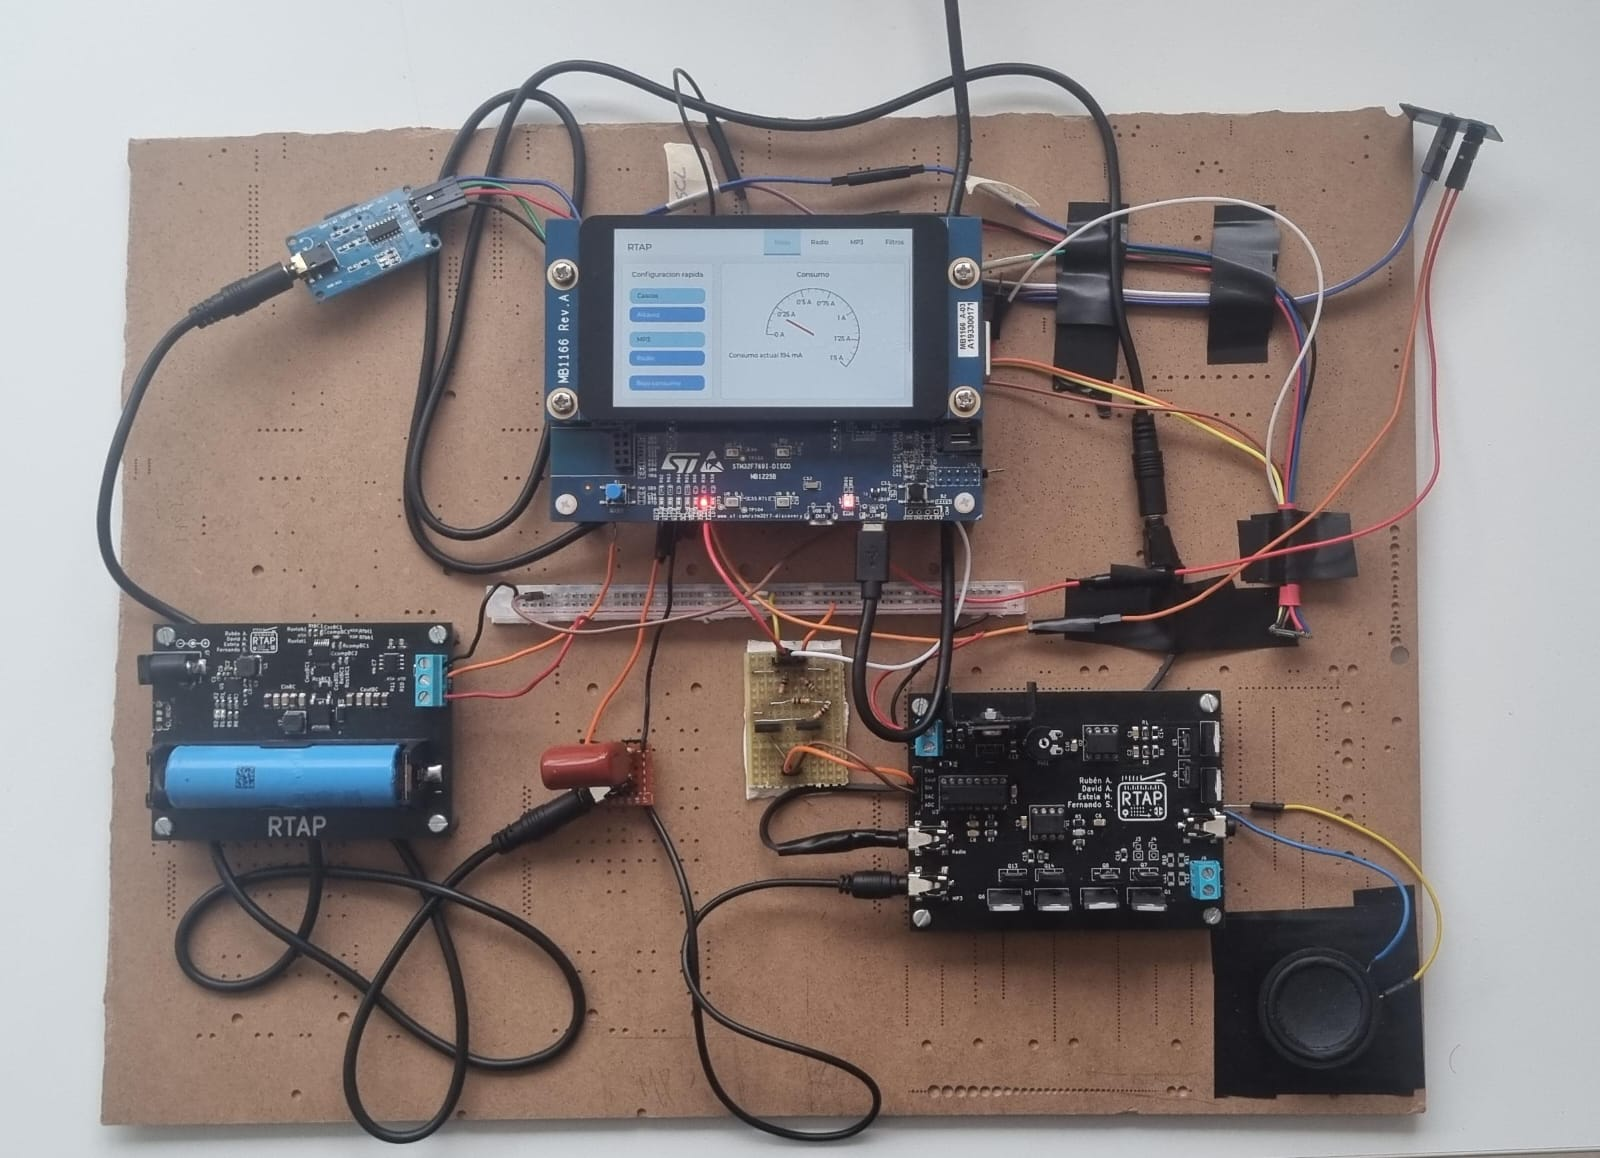
\includegraphics[width=\textwidth]{images/1/Foto_Sistema.jpg}
    \caption{Sistema Completo}
    \label{fig:1-Sistema_Completo}
\end{figure}
% \section{Desarrollo de subsistemas}

Para este proyecto hemos desarrollado dos subsistemas analógicos propios, sobre dos PCB distintas, una de alimentación y un amplificador de audio. Además, hemos utilizado tres subsistemas ya existentes para la recepción de audio, la reproducción de música en MP3 y la lectura de información NFC de un dispositivo móvil.

\subsection{La placa}
Para este proyecto se ha utilizado la placa \texttt{STM32F769NI-DISCO}, que es una placa de desarrollo comercializada por STM. Dispone de un procesador ARM Cortex M7, que puede funcionar a una frecuencia de hasta 216 MHz. 

Dispone de pines dispuestos de una forma adecuada para ser compatible con Arduino Uno.

Entre los periféricos presentes en la placa, los más importantes que utilizamos son:
\begin{itemize}
    \item \textbf{La pantalla:} Dispone de una pantalla LCD táctil de 4.3 pulgadas, accesible a través del periférico DSI, con una resolución de 800 x 480 píxeles, con una profundidad del  color de 16 bits, lo que resulta en un total de $2^{16}$ colores posibles de representar. En concreto, se asignan 5 bits para las componentes roja y azul, siendo los 6 restantes para la verde, que es la más importante.
    \item \textbf{La DMA2:} La pantalla restringe el uso de las DMA, siendo la 2 la única opción posible, puesto que es la única que tiene la opción de \textit{Memory-To-Memory}. Cualquier canal y flujo (\textit{Channel} y \textit{Stream}) son de libre elección.
    \item \textbf{Los ADCs:} La placa dispone tres ADCs, que funcionan a una frecuencia de 48 kHz, de los cuales nuestro proyecto utiliza dos: el ADC1 se utiliza para medir el consumo, y el ADC3 se utiliza como pin de entrada para el audio. 
    \item \textbf{El DAC:} La placa dispone de un DAC de 2 canales. En la documentación de la placa no se anuncia esta capacidad, únicamente se puede encontrar el la documentación del microcontrolador. El DAC también funciona a 48kHz, y se sincroniza con el ADC, como se explica en \autoref{para:temporizacion}.
    \item \textbf{El I2C:} Utilizamos un I2C para la comunicación con el módulo del NFC.
    \item \textbf{La SD:} Dispone de un puerto para introducir una tarjeta SD, a través del periférico SDMMC.
\end{itemize} 

\subsubsection{Algunas consideraciones}
En algunos proyectos, hemos intentado utilizar la sentencia \texttt{printf}, pero a priori parecía una tarea imposible. Revisando la documentación, constatamos que el pin \texttt{SW0} está desconectado en la configuración por defecto. Para que funcione dicha función, hay que soldar \texttt{R92}, que conecta \texttt{SW0} con el pin adecuado. Esta resistencia funciona como un jumper, ya que el valor anunciado por el fabricante es de 0 $\Omega$. Tras sujetar un cable de forma manual, conseguimos visualizar la salida de la \texttt{UART} desde el panel del debugger.
\subsection{Subsistema de alimentación}

El subsistema de alimentación es el encargado de permitir que el sistema se alimente a través de baterías. También permite cargar la batería e incluso ambas acciones simultáneamente.

Como batería hemos decidido utilizar una batería de ion de litio 18650, un modelo bastante estándar en las aplicaciones integradas.  Concretamente, hemos decidido utilizar el modelo \texttt{INR18650-29E} de Samsung, que tiene una tensión nominal de 3.7\ V y una capacidad de 2900\ mAh.

Sin embargo, este tipo de baterías tienen unos requisitos de carga muy estrictos. Contando con que la batería parte de un estado correcto (no por debajo del límite de tensión segura), se debe cargar primero con un método de corriente constante hasta alcanzar una tensión cercana a la máxima y después cambiar a un método de tensión constante hasta finalizar la carga \cite{BU409ChargingLithiumion}. Un ejemplo de ciclo de carga se puede ver en la \autoref{fig:2-1-cicloCarga}

\begin{figure}[h]
    \centering
    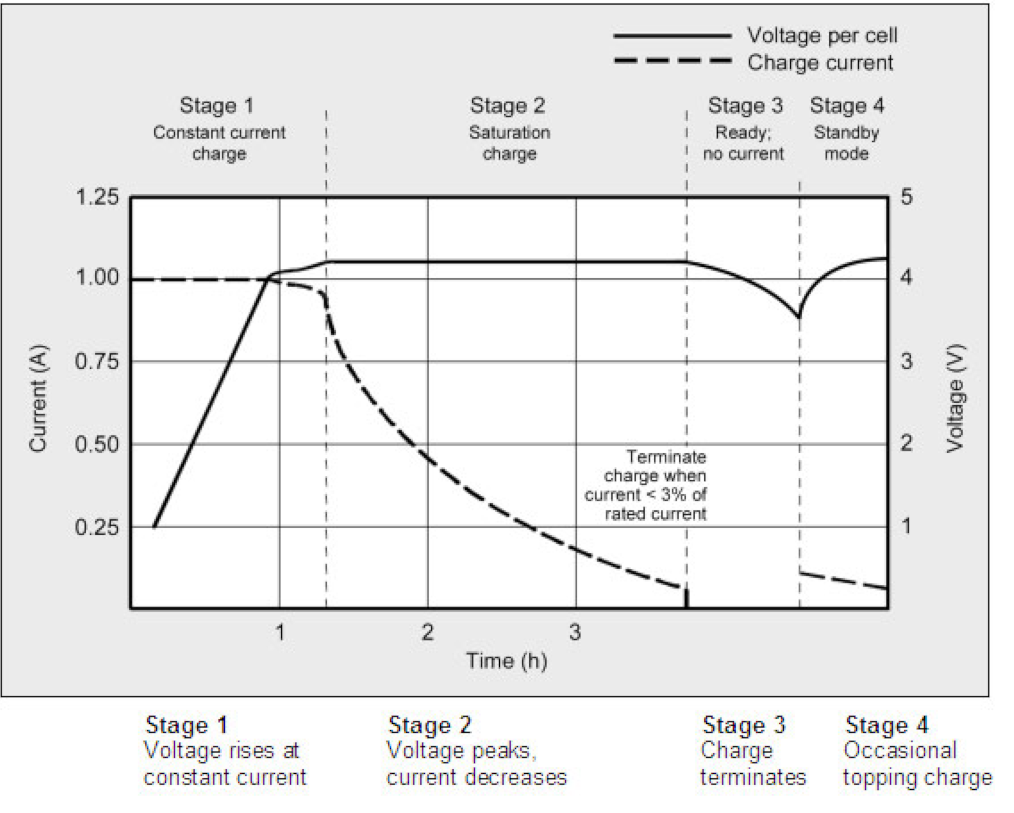
\includegraphics[width=0.5\textwidth]{images/2/2-1/cargaBateria.png}
    \caption{Ciclo de carga de una batería de ión de litio}
    \label{fig:2-1-cicloCarga}
\end{figure}

Si no se respeta el ciclo de carga de estas baterías, se tiene una alta probabilidad de que falle de forma violenta, siendo incluso un peligro de incendio. 

\subsubsection{Circuito de carga}

Para facilitarnos la tarea de respetar este ciclo hemos utilizado una solución integrada de Texas Instruments, el \texttt{BQ25606}, un cargador de una celda de litio que soporta hasta 3 amperios de corriente. \cite{BQ25606DataSheet}

Gracias a este circuito integrado y bastantes componentes externos, podemos diseñar un circuito que, a partir de una tensión de entrada entre 5 y 12 voltios y utilizando un convertidor reductor, carga la batería adecuadamente y de forma segura. 

La entrada al circuito puede ser a través de un conector \textit{Jack} de alimentación o un conector \textit{Micro USB}. Además, si se utiliza el segundo conector, el integrado se encarga de negociar el protocolo de carga rápida con la fuente de alimentación para incrementar la corriente de entrada y mejorar la potencia de carga. 

Además, si el circuito está conectado a la alimentación y la fuente tiene suficiente capacidad, la corriente de salida se obtiene de la entrada en lugar de la batería, gracias a la tecnología PowerPath de TI. Esta tecnología además permite balancear las tres corrientes, por lo que si el sistema requiriera de más corriente de la que la fuente de alimentación pudiera proveer, se obtendría también de la batería realizando un esfuerzo coordinado entre la fuente y la batería. Si por el contrario la fuente puede ofrecer más corriente de la que se está solicitando en la salida, se utiliza este excedente para cargar la batería.

Este circuito cuenta además con dos indicadores LED que informan sobre si la fuente de alimentación está conectada y las tensiones son correctas (verde en nuestro circuito) y si se está cargando la batería o hay algún fallo (roja en nuestro circuito). La segunda luz se mantiene encendida mientras se está cargando, se apaga cuando se ha finalizado la carga y parpadea a 1 Hz de frecuencia si hay algún error.

Para ofrecer todas estas características, el circuito integrado consta de una máquina de estados finitos y múltiples comparadores de error. Con esta inteligencia conmuta tres transistores para conectar la batería y para gestionar el convertidor conmutado síncrono que se construye. Se puede ver un diagrama de bloques resumido del circuito (obtenido de la hoja de catálogo) en la \autoref{fig:2-1-bloquesInternosBQ25606}

\begin{figure}[h]
    \centering
    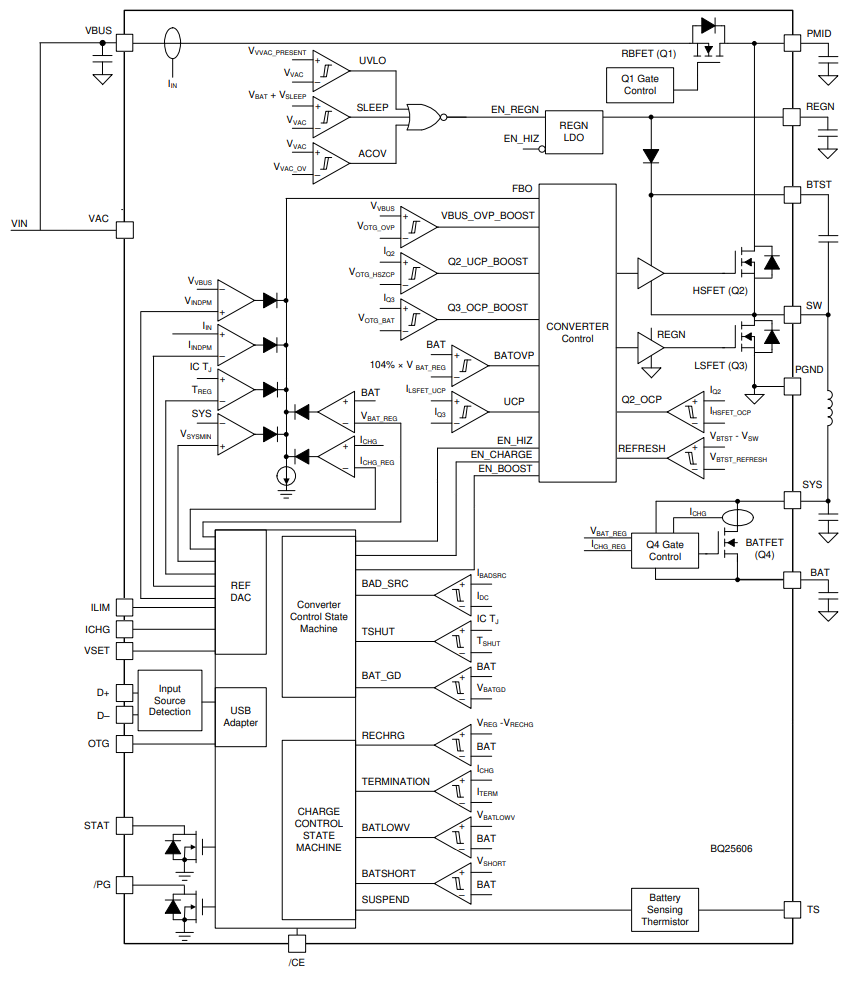
\includegraphics[width=0.5\textwidth]{images/2/2-1/BQ25606Bloques.png}
    \caption{Diagrama de bloques interno del BQ25606}
    \label{fig:2-1-bloquesInternosBQ25606}
\end{figure}

Este circuito ofrece a su salida una tensión aproximadamente igual a la de la batería durante el funcionamiento normal, por lo que está alrededor de los 3.7 V. Sin embargo, si la tensión de la batería cae por debajo de 3.5 V, el circuito se encarga de ofrecer dicha tensión a la salida, por lo que nunca bajará de dicho valor (mientras la batería puede ofrecer corriente y no esté descargada).

El circuito integrado ofrece también la posibilidad de utilizar una batería con sensor de temperatura integrado, pero no vamos a utilizarlo debido al incremento en coste de la misma.

En la hoja de catálogo del integrado se ofrece información sobre el proceso de diseño de un circuito alrededor de dicho integrado. Además, se tiene una nota de aplicación sobre el diseño de circuitos alrededor de este integrado \cite{texasinstrumentsDesigningStandaloneSingle}:

\begin{itemize}
    \item Inductancia de 2.2 $\mu$ F para reducir el rizado de corriente.
    \item Pin \texttt{VSET} flotante para tensión de carga máxima de 4.208 V.
    \item Divisor de tensión de dos resistencias de 10 $k\Omega$ en \texttt{TS} para no utilizar divisor de tensión.
    \item Resistencia de 165 $\Omega$ en \texttt{ILIM} para limitar la corriente de entrada cuando no se negocia carga rápida a 3 A (normalmente se utiliza mucho menos).
    \item Resistencia de 487 $\Omega$ en \texttt{ICHG} para limitar la corriente de carga máxima a 1.4 A como se indica en las especificaciones de la batería.
    \item El resto de componentes se toman de la Figura 10-1 de la hoja de catálogo
\end{itemize}

Por tanto, esta parte del circuito queda como se puede ver en la \autoref{fig:2-1-circuito-carga-final}.

\begin{figure}[h]
    \centering
    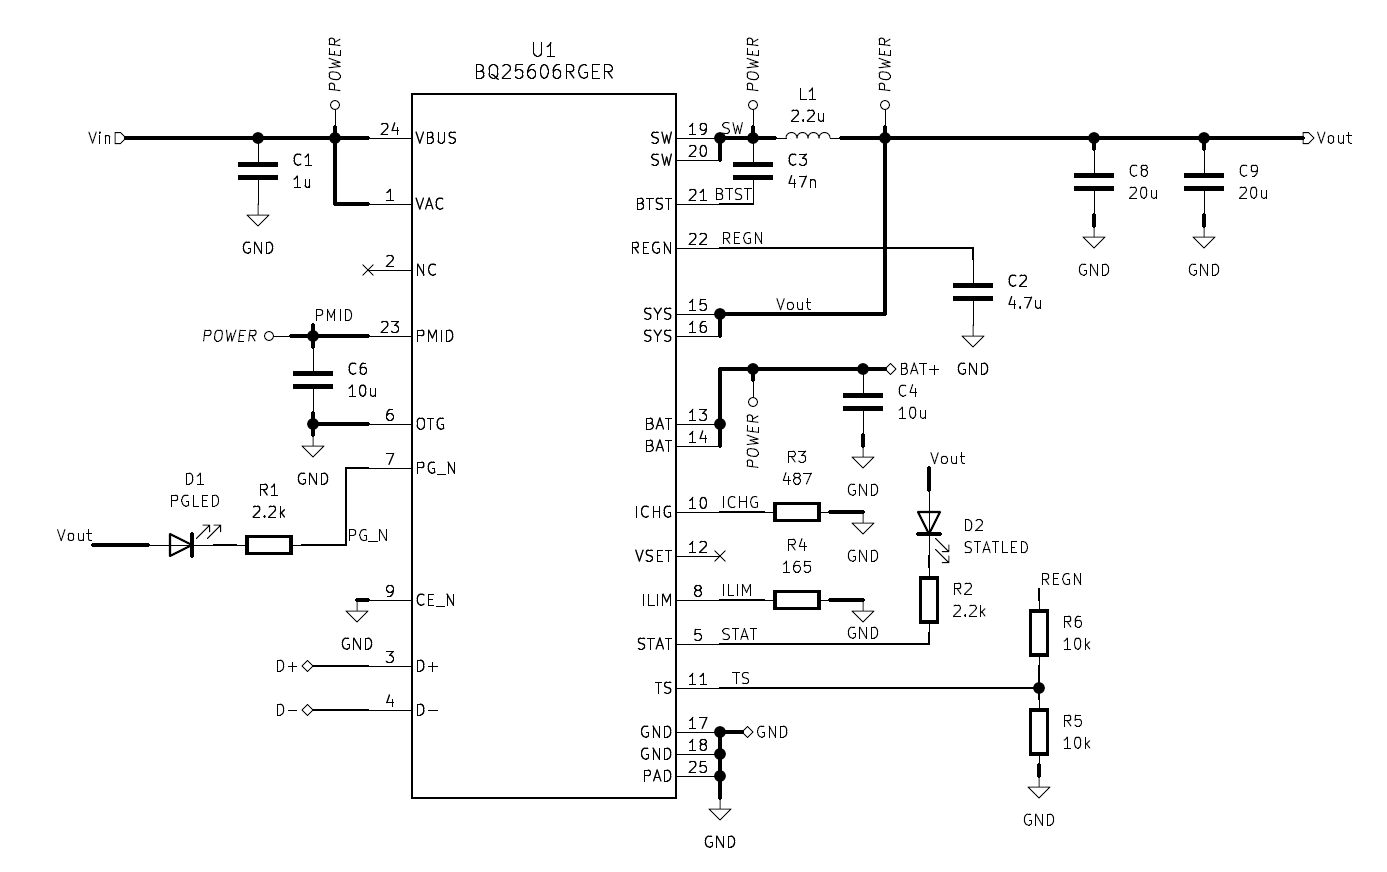
\includegraphics[width=\textwidth]{images/2/2-1/circuitoCarga.png}
    \caption{Subcircuito de carga de batería}
    \label{fig:2-1-circuito-carga-final}
\end{figure}

\subsubsection{Convertidor elevador}\label{subsubsec:convertidor_elevador}

La placa que utilizamos especifica una tensión de entrada de 7 V a 12 V si se utiliza el pin $V_{in}$ inferior. Preferimos utilizar este método ya que la entrada de 5 V no tiene protección y se puede dañar la placa si no se realiza todo el proceso adecuadamente.

Experimentalmente hemos notado que la placa utiliza la misma corriente de entrada para cualquier valor de tensión, por lo que seguramente utilice un convertidor de tensión lineal internamente para generar las tensiones. Por tanto, hemos preferido tomar el valor más pequeño de las tensiones de entrada para reducir la pérdida de potencia.

La tensión de salida del circuito de carga oscila entre los 3.5 V y los 4.2 V, por lo que hemos diseñado un convertidor conmutado elevador o \textit{Boost Converter} para obtener dicha tensión a partir de la salida del cargador.

Un circuito convertidor elevador está compuesto básicamente por una bobina, un transistor y un controlador PWM.\ Como controlador PWM hemos utilizado otra solución integrada de Texas Instruments debido a la alta precisión que nos permite tener, ya que un fallo en este circuito podría dañar seriamente al resto del sistema. 

El circuito integrado elegido es el LM51561H. Este circuito es un controlador de convertidores conmutados de tipo \textit{Boost, SEPIC} y \textit{Flyback} con gran rango de tensiones y muy elevada protección. \cite{LM51561HDataSheete}

Además, indica específicamente que está pensado para aplicaciones de batería gracias a su baja tensión de entrada necesaria para funcionar. Al contrario que el circuito del cargador, este integrado no incluye los transistores internos por lo que se tienen que añadir externamente. 

Este integrado consta básicamente de comparadores de error respecto a tensiones de referencia y un generador de señales triangulares para la generación de PWM. Cuenta además con la posibilidad de compensar el circuito para evitar su inestabilidad. La versión LM51561H es igual que la LM5156H solo que con protección en modo \textit{Hiccup}. En este modo de protección, si se detecta una sobrecarga, se desactiva el convertidor y se comienza una espera. Al finalizar la espera, se trata de volver a arrancar la conversión. Si la condición de sobrecarga sigue presente, se vuelve a dormir y repetir el ciclo. Esto permite una mucho menor potencia media en condición de sobrecarga en comparación a la protección por corriente media, pico o valle. \cite{hariImprovePowerConverter}

Se puede ver un diagrama de bloques resumido en la \autoref{fig:2-1-LM51561H-bloques}.


\begin{figure}[h]
    \centering
    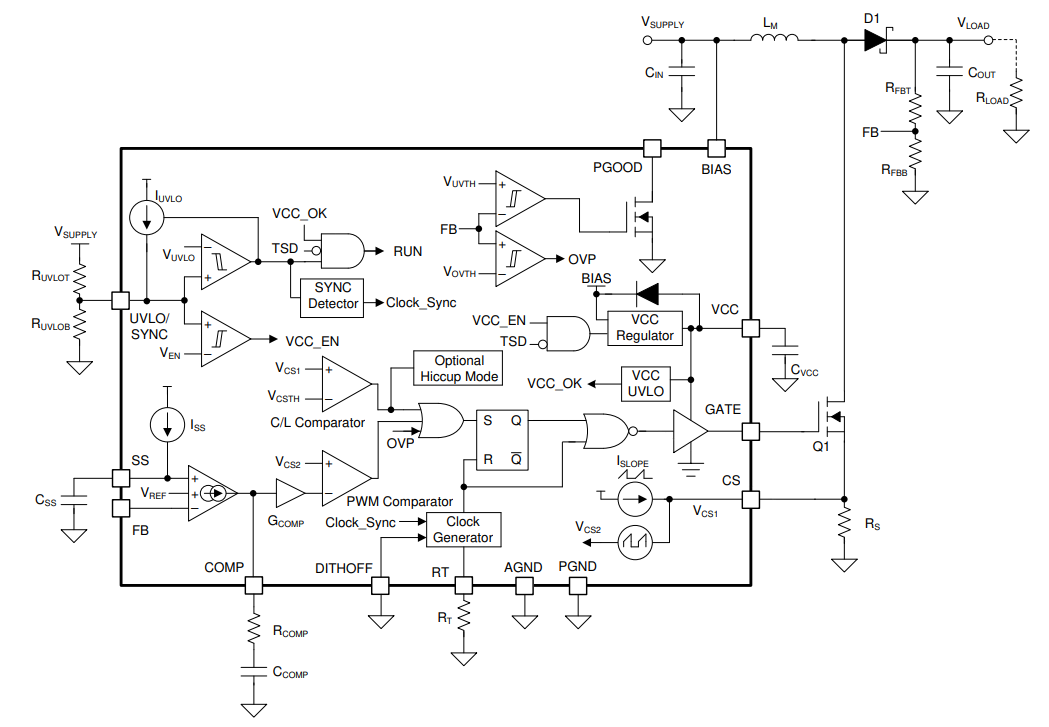
\includegraphics[width=0.5\textwidth]{images/2/2-1/LM51561HBloques.png}
    \caption{Diagrama de bloques interno del LM51561H}
    \label{fig:2-1-LM51561H-bloques}
\end{figure}

Algunas de las características destacables de nuestro circuito son:
\begin{enumerate}
    \item Protección contra infravoltaje (\textit{Undervoltage Lockout}). Se comprueba que el pin \texttt{UVLO} tenga una tensión superior a 0.55 V para comenzar la configuración interna y superior a 1.5 V para comenzar a conmutar.
    \item Frecuencia elevada de conmutación para evitar interferencias en las bandas de AM y reducir las pérdidas de conmutación.
    \item Salida de 7 V muy estable y con poca dependencia de la corriente de salida
\end{enumerate}

Para el diseño de este circuito, el fabricante recomienda el uso de la herramienta WEBENCH Power Designer\footnote{\url{https://www.ti.com/tool/download/SNVC224}}, que permite reducir la complejidad del diseño realizando los cálculos necesarios para los parámetros deseados y la compensación de la función de transferencia del circuito. 

Utilizando dicha herramienta, generamos el circuito que hemos utilizado con los siguientes parámetros: 
\begin{enumerate}
    \item $V_{in, \min} = 3.5\ V$
    \item $V_{in, \max} = 4.2\ V$
    \item $V_{out} = 7.0\ V$
    \item $I_{out} = 1.0\ A$
\end{enumerate}

Una vez introducidos los parámetros, el software genera el circuito con los componentes recomendados, permitiendo sustituirlos por equivalentes y generando las gráficas de funcionamiento aproximado. Se puede encontrar el reporte generado en el \autoref{anexo:webench-report}

Con el resultado de dicho software, se construye un circuito como el de la \autoref{fig:2-1-circuito-boost-final}.

\begin{figure}[h]
    \centering
    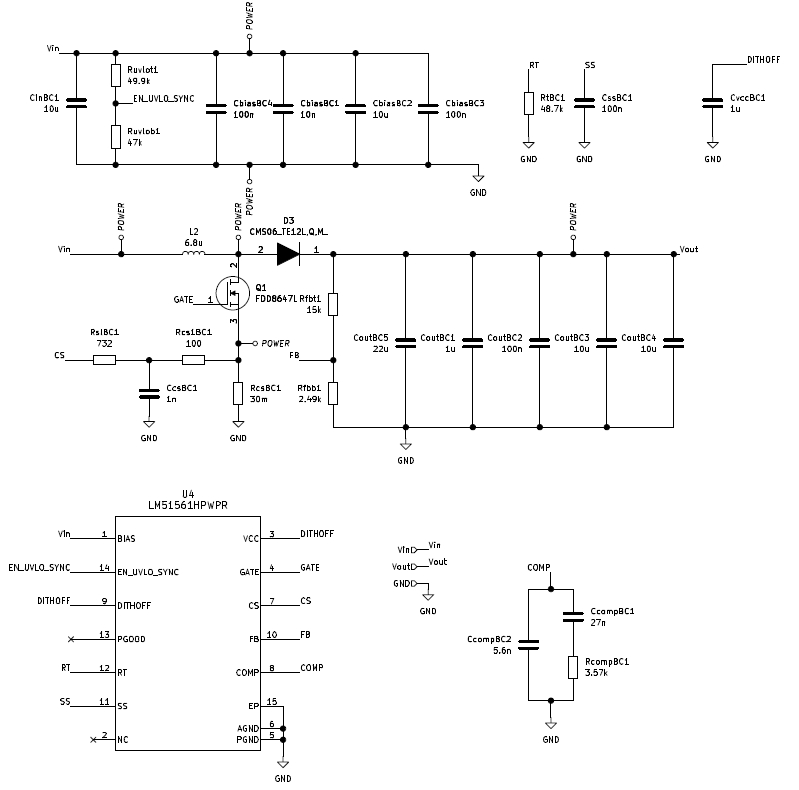
\includegraphics[width=0.5\textwidth]{images/2/2-1/circuitoElevador.png}
    \caption{Circuito del convertidor elevador}
    \label{fig:2-1-circuito-boost-final}
\end{figure}

\subsubsection{Medidor de consumo}
\label{subsubsec:medidor-consumo-analog}

Otra parte importante de este circuito es el medidor de consumo integrado. Para ello, primero pensamos en construir un amplificador de instrumentación, que se puede adquirir ya implementado en un mismo paquete o realizar con dos amplificadores operacionales. Sin embargo, durante la búsqueda de modelo de amplificador operacional encontramos un modelo que se ofrece como especializado en medición de corriente en el nivel bajo (\textit{Low-side current switching}) por lo que decidimos quedarnos con él.

Dicho integrado es el OPA187ID, un amplificador operacional de precisión con aproximadamente cero tensión de offset ($10\ \mu V$, $0.001\mu V/^\circ\! C$). \cite{OPA187DataSheet}

Dicho amplificador operacional recomienda montar una configuración de amplificador diferencial con una resistencia \textit{shunt} de muy baja impedancia y configurar la ganancia deseada mediante las resistencias de realimentación.

Como resistencia de medida hemos elegido un valor bajo, de $10\ m\Omega$ y que soporta 1 W de potencia. Para simplificar los cálculos, hemos decidido asignar el rango de entrada de un ADC de nuestra placa ($[0, 3.3]\ V$) a un rango de $[0, 3]\ A$. Por ello, la ganancia es:

\[
    G = \frac{3.3 - 0}{3 - 0} = 1.1 V/A  
\]

Para conseguir dicha ganancia es tan sencillo como utilizar resistencias con un cociente de 110, por lo que elegimos valores de $1\ k\Omega$ y $110\ k\Omega$ en el circuito, por lo que obtenemos el circuito de la \autoref{fig:2-1-medidor-consumo}.

\begin{figure}[h]
    \centering
    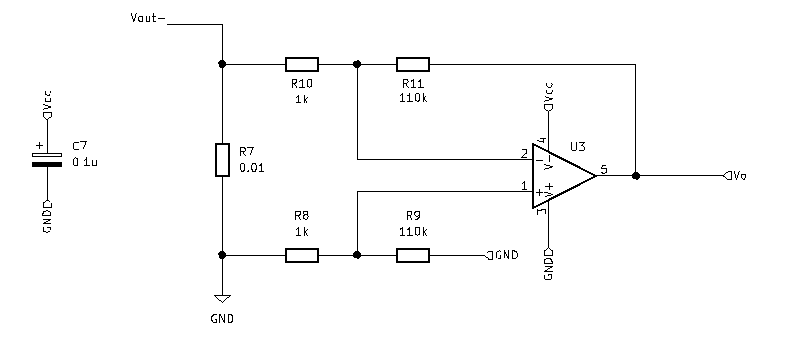
\includegraphics[width=0.5\textwidth]{images/2/2-1/circuitoConsumo.png}
    \caption{Circuito medidor de consumo}
    \label{fig:2-1-medidor-consumo}
\end{figure}

\subsubsection{Diseño de PCB}

Los tres circuitos se han integrado en una sola PCB, permitiendo una mucho mejor integración y uso mucho más sencillo. Se ha integrado un zócalo para insertar la batería sobre la placa y evitar la posibilidad de una mala conexión. Además, se han incluido los conectores de entrada de potencia previamente mencionados, tanto el Jack de alimentación como el conector micro-USB. Por otro lado, la salida del sistema se realiza a través de unos terminales de tornillo que incluyen la tensión de alimentación positiva, negativa y la medida de consumo.

Sin embargo, por un problema durante el ensamble de la placa, se destruyeron los pads del conector micro-USB, por lo el conector no funciona correctamente. Sin embargo, el sistema funciona perfectamente a través del Jack de alimentación.

La alta complejidad de los circuitos integrados hace que sus empaquetados sean muy pequeños, por lo que la soldadura se ha tenido que realizar mediante horno y con stencil. Sin embargo, esto nos ha permitido colocar los componentes muy próximos entre sí, reduciendo el ruido electromagnético generado y las componentes parásitas del circuito. Concretamente, el circuito integrado de carga es de empaquetado \texttt{VQFN24} con un tamaño de $4x4\ mm$ y el integrado del conversor es \texttt{HTSSOP14} con un tamaño de $5x4.4\ mm$.

Además, el pequeño tamaño de estos circuitos reduce significativamente su capacidad de disipación térmica. Por ello, ambos incluyen un pad en su parte inferior que debe ser soldado a un pad que además incluya muchas vias térmicas a la capa inferior, en la que debe haber un plano de tierra grande para disipar el calor que se genere. Por ello y para ofrecer un camino de retorno a las altas corrientes que recorren este circuito, la capa inferior se dedica casi exclusivamente a la masa del circuito. 

Ambos circuitos integrados ofrecen indicaciones sobre la disposición de los componentes que se han seguido rigurosamente. Por ejemplo, se recomienda mantener los bucles de conmutación lo más pequeños posibles o mantener separadas las tierras digital y analógica, juntandolas únicamente en un punto. 

Ciertas zonas del circuito han tenido que ser diseñadas mediante polígonos especiales al no poderse realizar la conexión mediante pistas normales o necesitar zonas especialmente grandes para caminos de mucha corriente.

Se puede ver el resultado final del circuito de alimentación en la \autoref{fig:2-1-circuito-alimentacion}.

\begin{figure}[h]
    \centering
    \includegraphics[width=0.5\textwidth]{images/2/2-1/circuitoAlimentación.jpg}
    \caption{Circuito de alimentación}
    \label{fig:2-1-circuito-alimentacion}
\end{figure}

Se tiene un esquema completo del circuito en el \autoref{anexo:circuito-alimentacion}
\clearpage
\subsection{Subsistema de audio}

El subsistema analógico de audio tiene tres funciones principales:
\begin{enumerate}
    \item Multiplexar las dos entradas de audio (MP3 y Radio) a un ADC del microcontrolador
    \item Multiplexar la salida proveniente del DAC a una de las dos salidas de audio (Altavoces o auriculares)
    \item Amplificar la salida de audio seleccionada
\end{enumerate}

\subsubsection{Divisor de rail}
Este sistema se alimenta directamente desde el módulo de alimentación explicado en el apartado anterior. Por ello, cuenta con una entrada unipolar de 7 voltios. Sin embargo, los circuitos de audio necesitan alimentación bipolar para funcionar. Por ello, hemos decidido implementar un circuito divisor de rail, que genera una tensión intermedia que se utilizará como nueva referencia del circuito, obteniendo una alimentación virtual de $\pm$3.5 V.

El circuito utilizado es un divisor de tensión de precisión implementado mediante el amplificador operacional \texttt{OP07}. Este amplificador operacional tiene muy bajo error estático y además cuenta con dos terminales para el ajuste del offset mediante un potenciómetro, por lo que es ideal para nuestra aplicación.

Sin embargo, los amplificadores operacionales permiten muy poca corriente a través de su terminal de salida, por lo que se necesita un circuito que permita incrementar la corriente de salida o entrada de dicho circuito sin afectar demasiado a la salida. Para ello, se utiliza una topología \textit{Push-Pull} en la que se utilizan dos pares de Darlington, es decir, cuatro transistores, para incrementar la capacidad de corriente del circuito. 

Al introducirlos dentro del lazo de realimentación, se elimina el efecto de las tensiones de base y se elimina el ruido que pudieran introducir, pero a cambio introducen la posibilidad de inestabilizar el circuito. Teniendo esta posibilidad en cuenta, incluimos la posibilidad de soldar un condensador entre el terminal de salida del amplificador y la alimentación negativa del circuito, para introducir un polo que compense la estabilidad. Sin embargo, hemos acabado no necesitando utilizarlo. 

Por tanto, el circuito generador de tierra virtual o divisor de rail queda como se puede ver en la \autoref{fig:2-2-tierra-virtual}.

\begin{figure}[h]
    \centering
    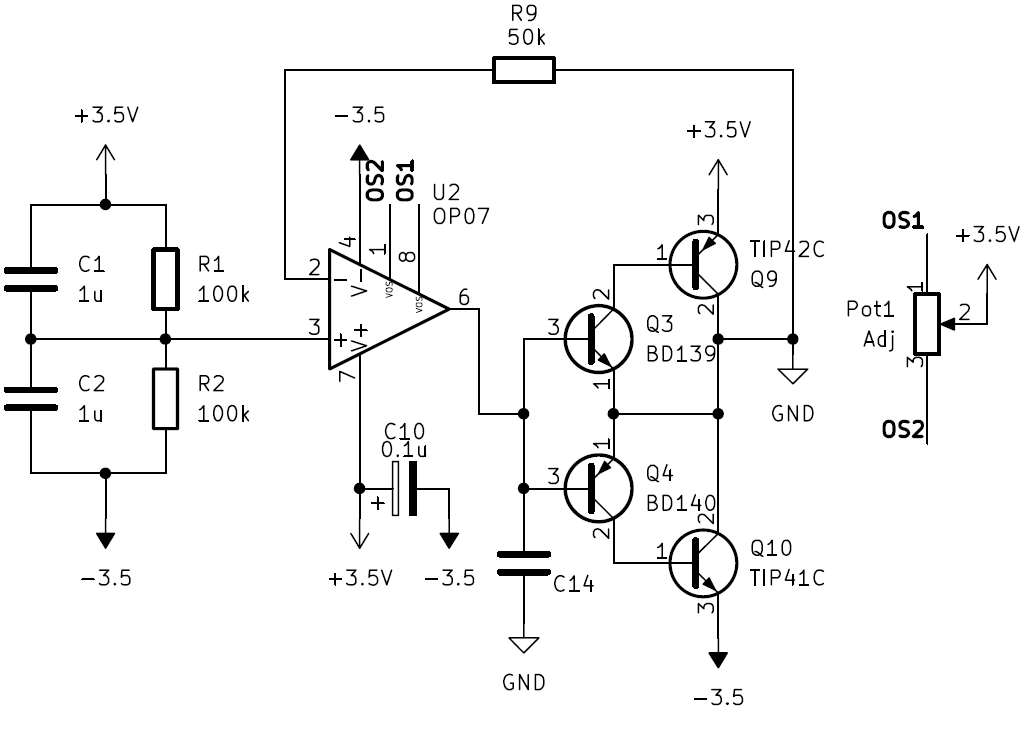
\includegraphics[width=0.5\textwidth]{images/2/2-2/circuitoDivisorRail.png}
    \caption{Circuito divisor de raíl}
    \label{fig:2-2-tierra-virtual}
\end{figure}

\subsubsection{Habilitación del circuito}

Para eliminar el consumo parásito del circuito cuando el sistema entre en el modo bajo consumo, se ha implementado un subcircuito de habilitación el cual permite encender o apagar el resto de subsistema (aunque finalmente el consumo parásito es muy pequeño).

Dicho circuito consiste en un transistor MOSFET de canal N en la alimentación, que permite cortar o dejar pasar la alimentación. Además, la baja impedancia de conducción del transistor permite que no haya casi pérdidas de potencia en el transistor. Sin embargo, ya que para cortar el transistor se necesita polarizar la puerta con una tensión próxima a 7 voltios y soportar las corrientes de los transitorios de conmutación, se utiliza otro transistor con una resistencia de \textit{pull-up} para adaptar los niveles los GPIO y reducir la corriente necesaria. Esto tiene el efecto añadido de invertir la polaridad de la habilitación que junto a la inversión del canal N se anulan, provocando que un nivel alto en el GPIO habilite el circuito. 

Por tanto, el circuito final es el que se ve en la \autoref{fig:2-2-circuito-habilitacion}.

\begin{figure}[h]
    \centering
    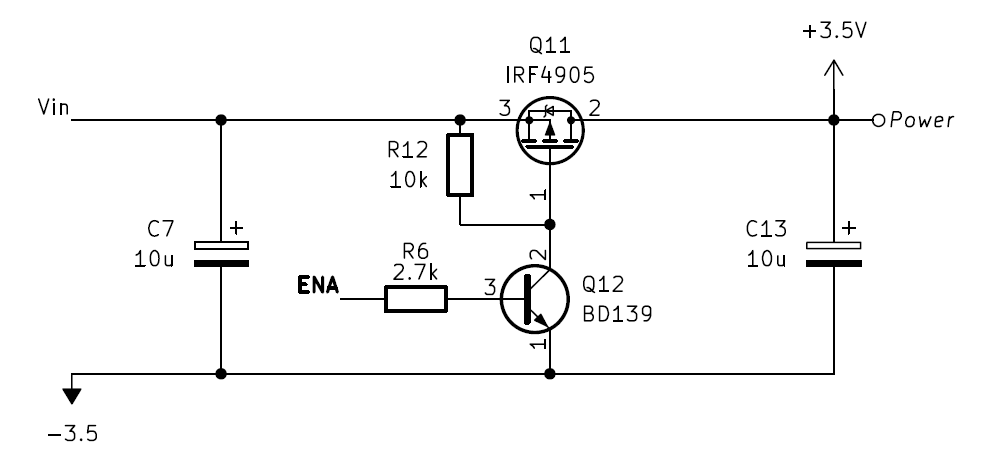
\includegraphics[width=0.5\textwidth]{images/2/2-2/circuitoHabilitacion.png}
    \caption{Circuito de habilitación}
    \label{fig:2-2-circuito-habilitacion}
\end{figure}

\subsubsection{Multiplexación de audio}

Para la multiplexación de audio se va a utilizar un multiplexor integrado. Inicialmente tratamos de diseñar un circuito que multiplexara los caminos de audio mediante componentes discretos, encontrando la estructura de la Puerta de Transmisión \cite{TransmissionGate}, como la que se puede ver en la \autoref{fig:2-2-puerta-transmision}

Sin embargo, todas las estructuras discretas que encontramos necesitan una familia de transistores de efecto de campo en los que el canal no está unido internamente al sustrato, permitiendo cargar la capacidad puerta-canal sin afectar a la tensión del camino drenador-surtidor. 

El principal problema de estos transistores es su elevado precio y muy poca variedad, siendo casi imposible encotrarlos. Además, generalmente se utilizan en aplicaciones de alta potencia por lo que su rendimiento para aplicaciones de baja señal suele ser bastante pobre.

\begin{figure}[h]
    \centering
    \includegraphics[width=0.3\textwidth]{images/2/2-2/puertaTransmisión.png}
    \caption{Puerta de transmisión con transistores con canal desconectado}
    \label{fig:2-2-puerta-transmision}
\end{figure}

Finalmente, descartamos la idea de utilizar componentes discretos y utilizamos una solución integrada. Por tanto, utilizamos el multiplexor analógico \texttt{CD4053BC}. \cite{CD4053BDataSheet}

Este multiplexor cuenta con tres canales en configuración \texttt{SPDT}, por lo que cada canal tiene un terminal en un extremo y dos en el otro. Este multiplexor cuenta con la ventaja de ser bidireccional, cosa de la que muchos otros carecen y es fundamental para nuestra funciononalidad.

Este multiplexor se utiliza para conectar las dos entradas de audio, que provienen de conectores Jack de audio de 3.5 mm a un GPIO que se conecta internamente a un ADC de la placa y para conectar otro GPIO que se conecta internamente a un DAC a las entradas de los dos caminos de amplificación de audio. 

\subsubsection{Cambiador de nivel lógico}

Un error que cometimos es no tener en cuenta la tensión de habilitación necesaria para conmutar un canal del multiplexor, por lo que los 3.3V de salida de un GPIO no son suficientes para cambiar el canal del multiplexor. Esto provoca que se esté siempre seleccionado el canal correspondiente al nivel bajo.

Para solucionar esto, hemos construido un circuito cambiador de nivel lógico que adapta los 3.3 V de la placa a los 7 V necesarios para conmutar el multiplexor (realmente el mínimo es aproximadamente 5V).

La solución que hemos pensado consiste en un inversor lógico TTL, que consiste en un transistor bipolar NPN con una resistencia de \textit{Pull-up}. La única desventaja es la inversión de nivel, pero se corrige fácilmente en el software.

Se puede ver el diagrama de nuestra solución en la \autoref{fig:2-2-cambiador-nivel}, en la que se muestra un cambiador. Hemos soldado dos de ellos en una placa de prototipado, que se puede ver en la \autoref{fig:2-2-foto-cambiador}.

\begin{figure}[h]
    \centering
    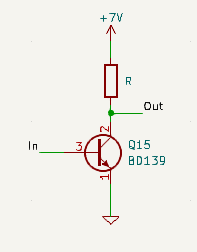
\includegraphics[width=0.5\textwidth]{images/2/2-2/circuitoCambiadorNivel.png}
    \caption{Circuito cambiador de niveles}
    \label{fig:label}
\end{figure}

\begin{figure}[h]
    \centering
    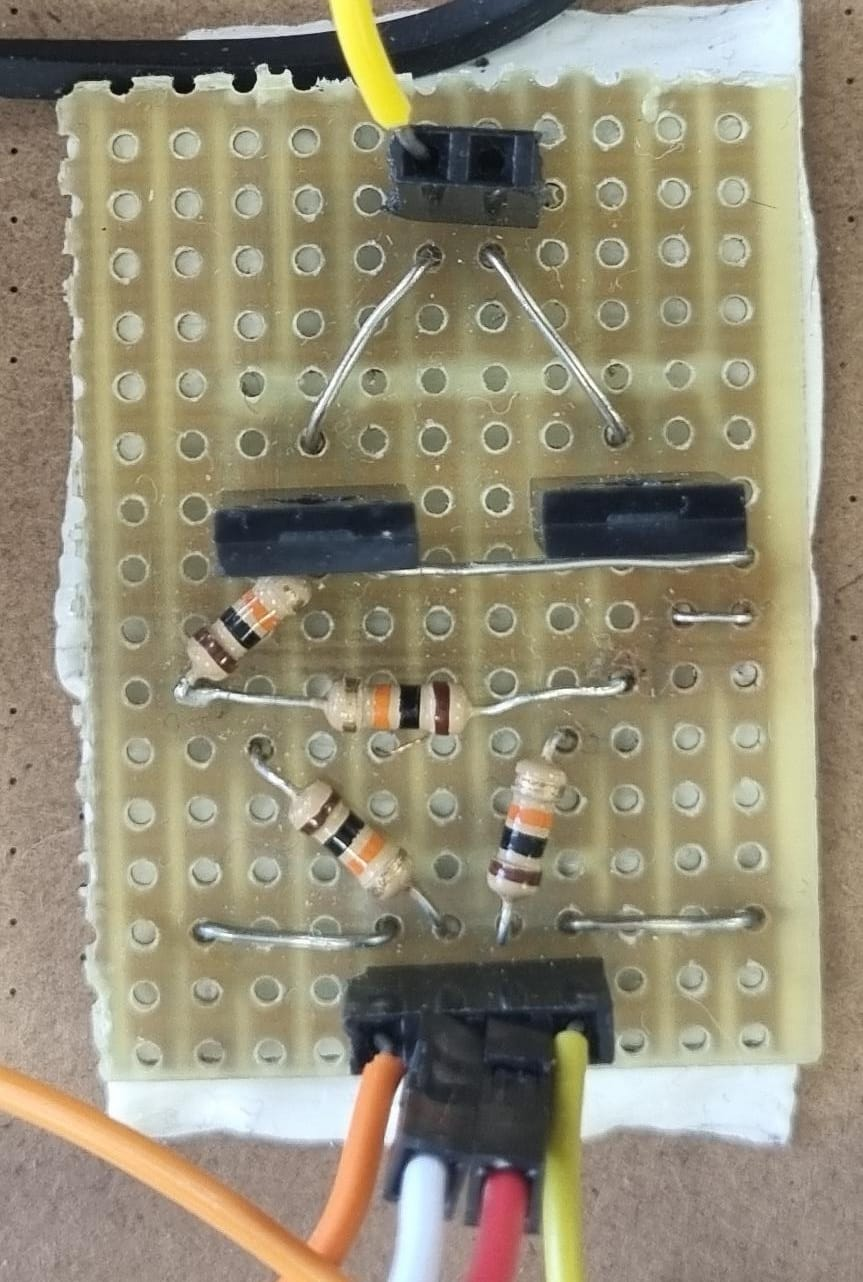
\includegraphics[width=0.25\textwidth]{images/2/2-2/cambiadorNivel.jpg}
    \caption{Foto del circuito cambiador de nivel}
    \label{fig:2-2-foto-cambiador}
\end{figure}
\subsubsection{Amplificador de audio para los auriculares}

La salida del DAC de la placa es una señal entre 0 y 3.3 V con 12 bits de resolución. Por tanto, el audio que se genere tiene una componente continua que se debe eliminar. 

Para eliminar esta componente continua hemos implementado una configuración de filtro paso alto mediante un filtrado pasivo y un seguidor de tensión realizado con un amplificador operacional. En el camino de realimentación del amplificador operacional se coloca una resistencia para anular la tensión de error de \textit{offset} del amplificador operacional.

También se añade la misma estructura de transistores que en el circuito generador de tierra virtual, que ahora al estar también dentro del lazo de realimentación cuentan con la ventaja de que se anula la distorsión de cruce. 

Los valores elegidos para los componentes del filtro son una resistencia de $100\ k\Omega$ y un condensador de $100\ nF$. Con ello, conseguimos una frecuencia de corte de:

\[
    f_c = \frac{1}{2\pi RC} \approx 16\ Hz    
\]

Elegimos este valor ya la banda de audición humana máxima es de $20$ Hz a $20$ kHz.

Se puede ver un diagrama de la solución que montamos en la \autoref{fig:2-2-amp-cascos}.

\begin{figure}[h]
    \centering
    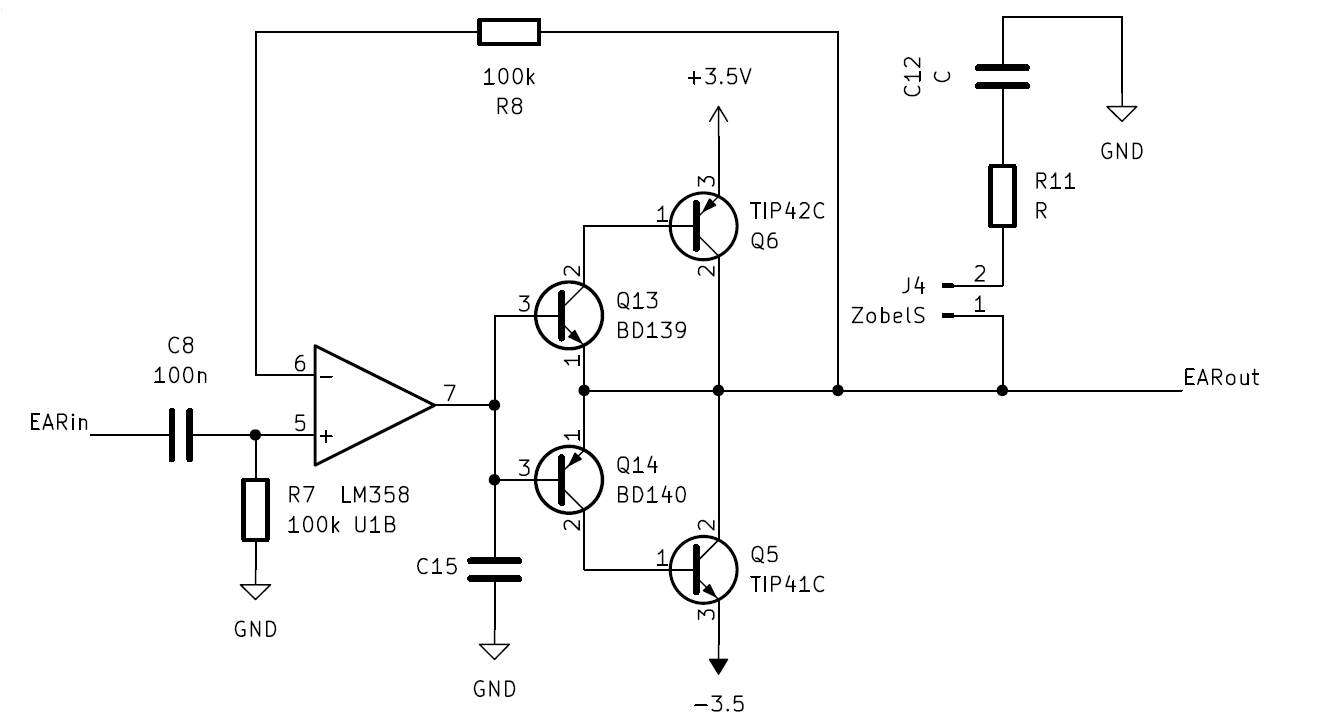
\includegraphics[width=0.7\textwidth]{images/2/2-2/circuitoAmplificadorCascos.png}
    \caption{Circuito amplificador de auriculares}
    \label{fig:2-2-amp-cascos}
\end{figure}

Sin embargo, al montar y probar el circuito detectamos que tenía un problema de inestabilidad para una frecuencia, lo cual es un problema común en los circuitos realimentados. Esto ocurre ya que la introducción del los transistores añade modificaciones impredecibles a la ganancia de lazo, provocando un muy molesto zumbido en los altavoces.

La solución que encontramos a este problema es la realimentación parcial mediante un condensador entre la salida del amplificador operacional y la base de los transistores. El tamaño del condensador afecta directamente a la reducción del ruido, cuanta más capacidad mejor lo elimina ya que hace una realimentación más directa. Sin embargo, cuanta mayor capacidad se le aplique, más se aprecia el efecto de la distorsión de cruce, la cual era eliminada al hacer la realimentación a la salida.

Experimentalmente probamos valores distintos determinando que el mejor balance entre ruido y distorsión de cruce se tiene para un valor aproximado de $33 \mu F$. Sin embargo, este valor no es propio del circuito sino de las tolerancias y efectos parásitos de los componentes, por lo que podría variar mucho según las circunstancias.

Otra cuestión a la que nos enfrentamos es la cantidad de canales. Inicialmente diseñamos el circuito para ofrecer un solo canal de audio y dirigirlo a ambos canales, pero se pierde bastante calidad por lo que decidimos dejarlo en audio por un solo canal. Si se quisiera obtener audio por ambos canales o incluso estéreo, se debería duplicar este circuito y colocar uno por canal.

\subsubsection{Amplificador de altavoces}

El circuito amplificador de altavoces cuenta con el mismo paso bajo que el amplificador de los auriculares, pero se utiliza otra resistencia para aportar ganancia al circuito. Además, ya que se introduce la rama a tierra se añaden un par de condensadores para realizar un filtrado de alta frecuencia y eliminar el ruido debido a la tensión y corrientes de offset.

La frecuencia de corte del filtro paso bajo es de:
\[
    f_c = \frac{1}{2\pi RC} \approx 21.2\ kHz
\]

Elegida igualmente para eliminar las frecuencias fuera del espectro auditivo humano.

La ganancia se elige para convertir el rango de salida ideal del DAC ($[0, 3.3]\ V$) en el rango máximo ideal de los amplificadores antes de la saturación ($[0, 7]\ V$) aunque la señal de audio no va a llenar el fondo de escala por su reducida amplitud. Por tanto, se elige una ganancia de tensión de:

\[
    A_v = 1 + \frac{R_4}{R_5} = 1.91 V/V
\]

Al igual que los otros dos circuitos, se introducen los transistores en el lazo de realimentación para la corriente, aunque en este caso no es necesario el condensador de realimentación parcial. Se tiene un esquemático de este subcircuito en la \autoref{fig:2-2-amp-altavoz}.

\begin{figure}[h]
    \centering
    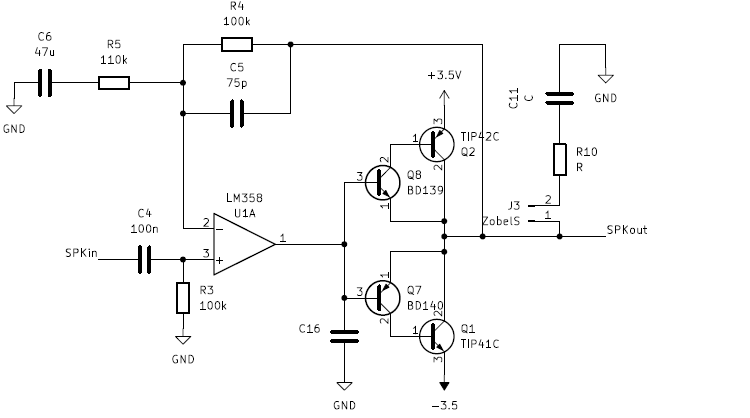
\includegraphics[width=0.7\textwidth]{images/2/2-2/circuitoAmplificadorAltavoces.png}
    \caption{Circuito amplificador de altavoces}
    \label{fig:2-2-amp-altavoz}
\end{figure}

\subsubsection{Diseño de PCB}

Todos estos sistemas se han integrado en una única PCB para intentar maximizar la integridad de la señal de audio, lo cual se consigue totalmente si se conecta el circuito sin tener en cuenta el \autoref{subsec:entre-dos-tierras}.

Hemos utilizado conectores Jack hembra de 3.5 mm para las dos entradas de audio y la salida a los auriculares. Un problema de este tipo de conectores es que el número de anillos puede variar en función de si los auriculares tienen o no micrófono y si son mono o estéreo. Si se quiere utilizar unos auricules con micrófono con nuestro sistema, se deben dejar ligeramente extraidos del conector para que haga mejor contacto la banda de tierra y mejorar significativamente el sonido.

La salida de altavoz se realiza a través de un terminal de dos tornillos para facilitar su conexión.

Como ya hemos comentado anteriormente, el circuito de transistores cuenta con un condensador de estabilizacion que finalmente no hemos utilizado. 

Además, hemos añadido la posibilidad de utilizar una red de Zobel, circuito que sirve para linealizar la respuesta en frecuencia de la inductancia intrínseca de los altavoces mediante un capacitor y una resistencia, pero finalmente no la hemos necesitado, por lo que tampoco está soldada.

El circuito cuenta además con un potenciómetro que sirve para ajustar el offset de la tensión de la tierra virtual gracias a los terminales específicos del \texttt{OP07}.

Hemos utilizado componentes SMT para los componentes pasivos y los conectores de audio y THT para los circuitos integrados, transistores y conectores de terminal.

Se puede ver una imagen del circuito finalizado en la \autoref{fig:2-2-circuito-foto} y el esquemático completo en el \autoref{anexo:circuito-audio}.

\begin{figure}[h]
    \centering
    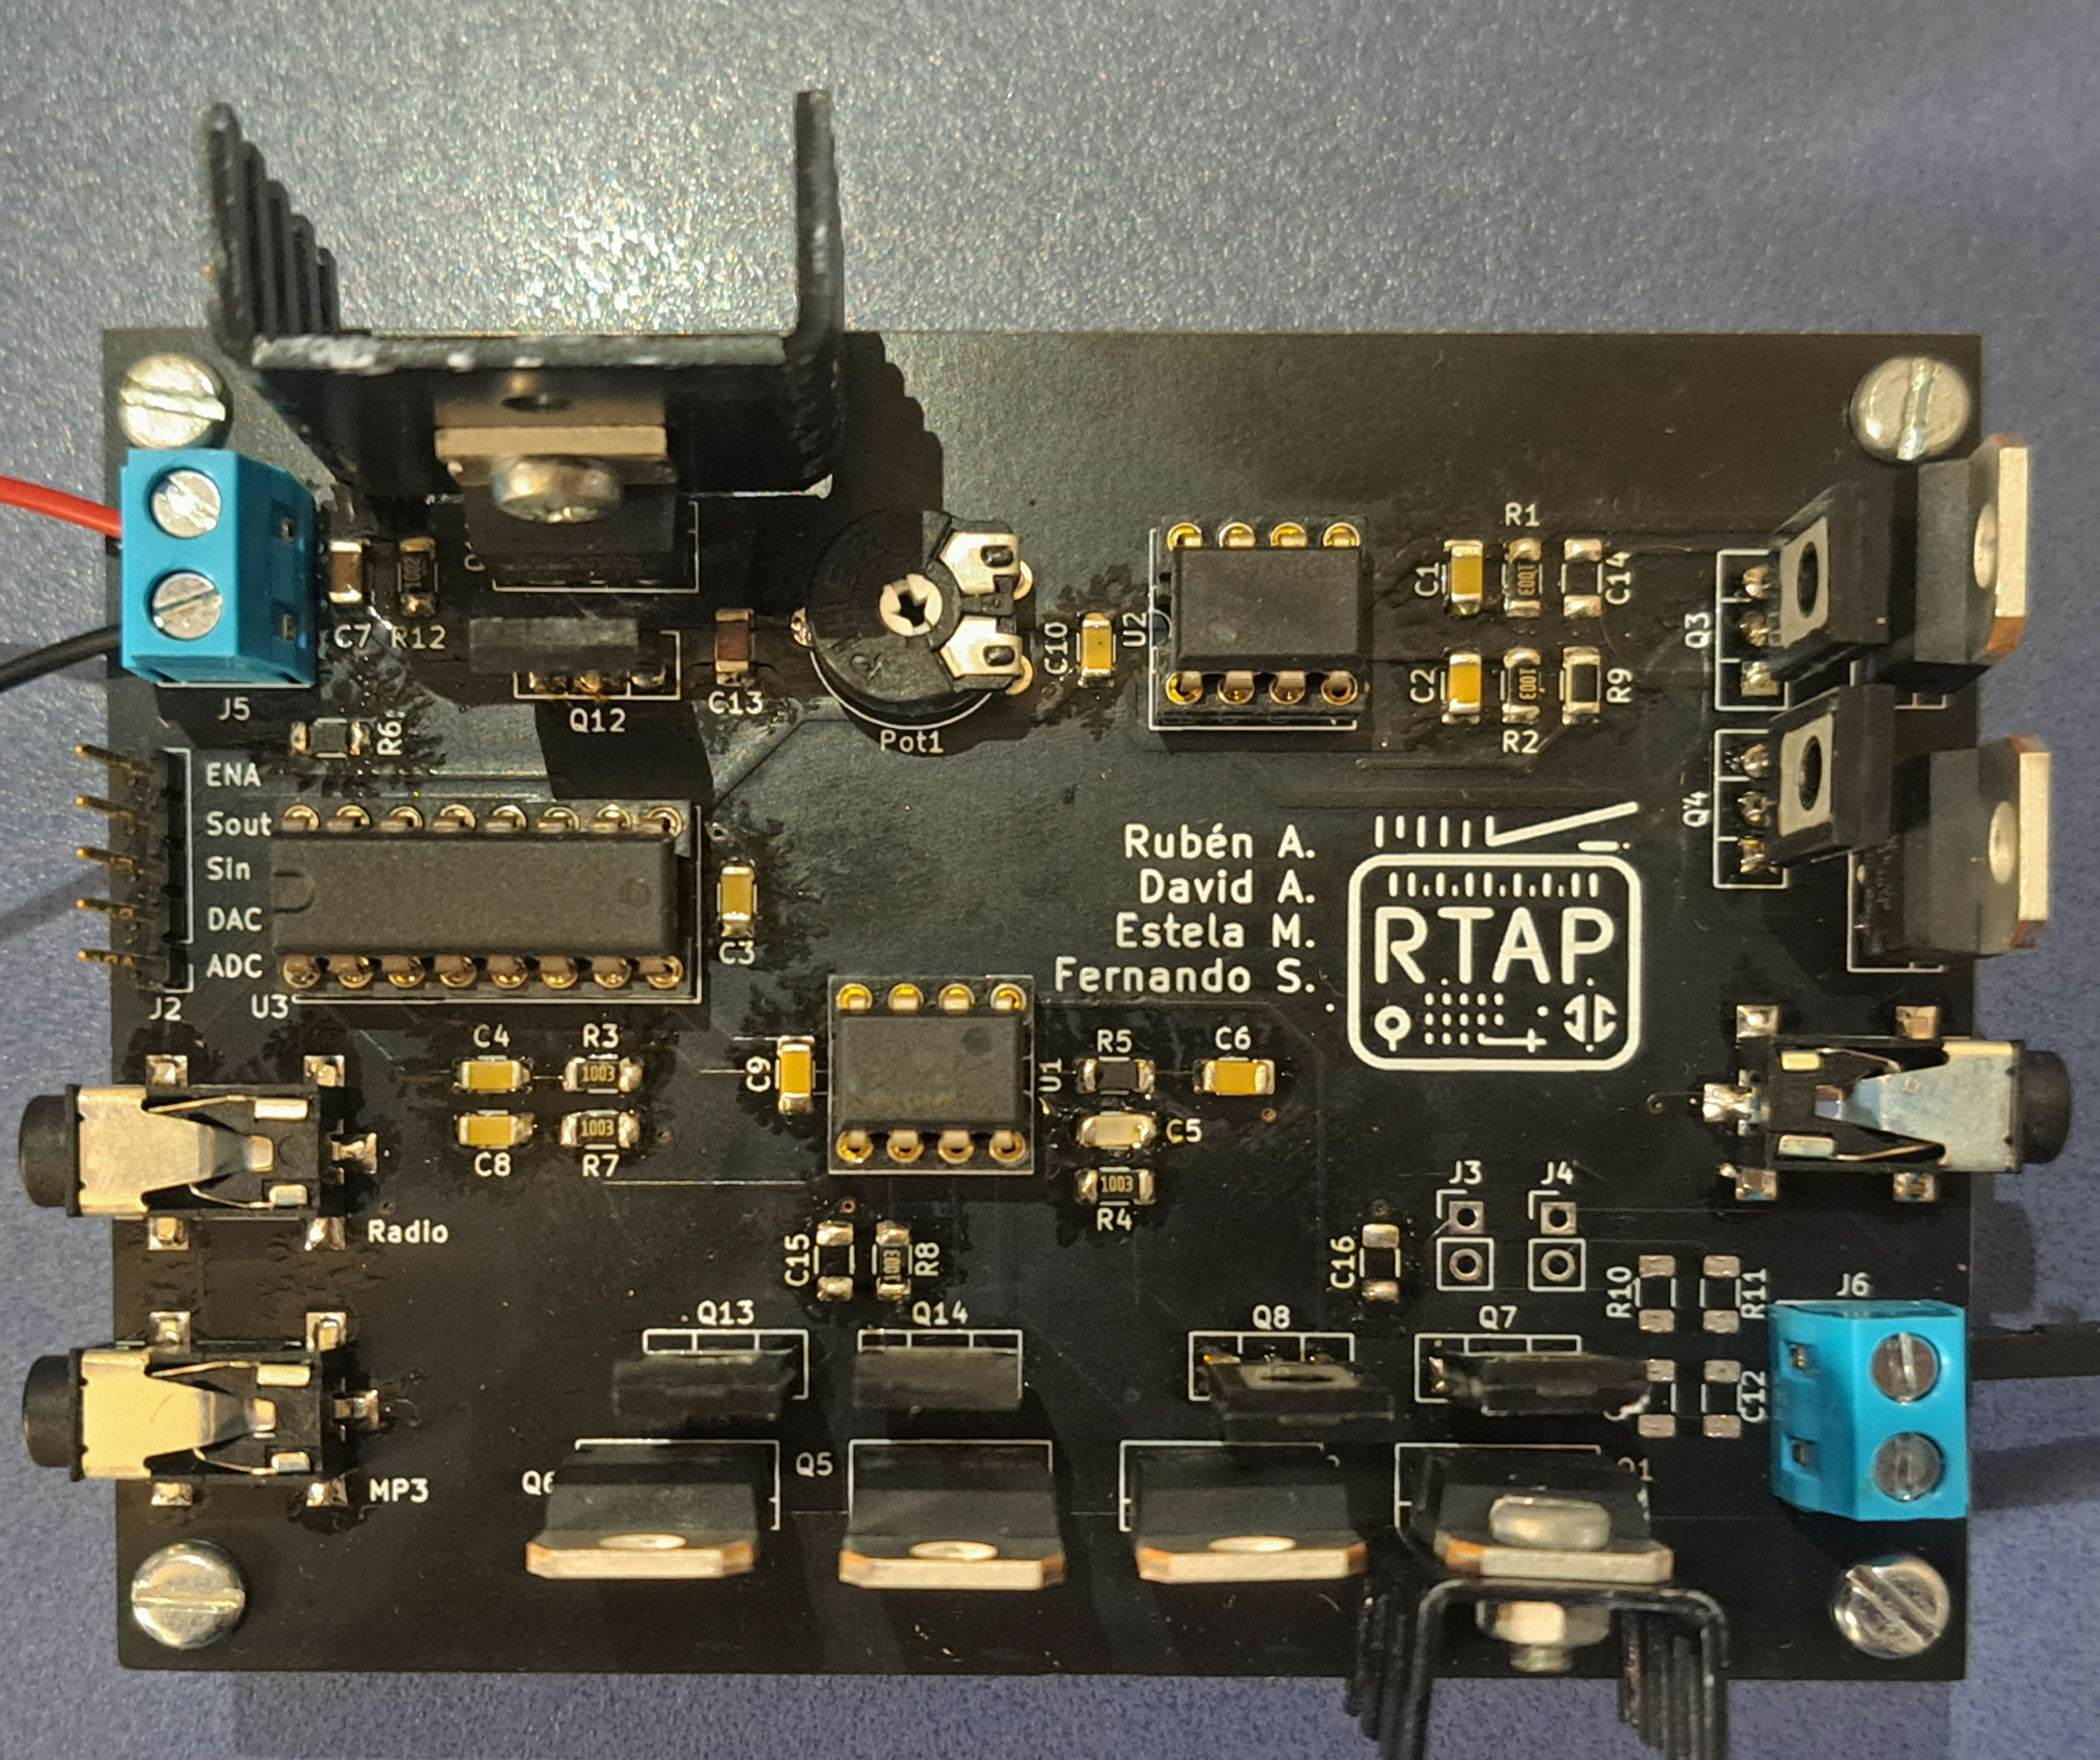
\includegraphics[width=0.5\textwidth]{images/2/2-2/circuito-foto.jpg}
    \caption{Circuito de audio completo}
    \label{fig:2-2-circuito-foto}
\end{figure}
\subsection{Módulo de radio}
El modelo de radio elegido ha sido el Sintonizador FM RDA5807M, mostrado en la \autoref{fig:2-3-Radio},  utilizado anteriormente en la asignatura de Sistemas Basados en Microprocesadores.

Dicho modelo se comunica con el microcontrolador mediante el protocolo \texttt{I2C}. El sintonizador cuenta con un decodificador MPX, salida de audio stereo y un rango de sintonización de 87 MHz a 108 MHz debido a nuestra situación geográfica.

En cuanto a la señal de audio de salida, hemos encontrado que presenta una componente continua de 1.65V y una amplitud de aproximadamente 1V. Debido a la conectividad que presenta el sintonizador, nos hemos encontrado el problema de que, al unirlo junto al resto del proyecto, cortocircuita la señal de masa analógica con la señal de masa virtual creada en nuestro circuito. Dicho problema se comentará en el \autoref{subsec:entre-dos-tierras}.

Por otra parte, necesita ser alimentado con una tensión entre 1.8V y 3.3V, soporta una corriente máxima de 10mA, cuenta con una relación señal-ruido típica de 55dB y presenta una distorsión armónica de audio total máxima del 0.2\%.

Todas las características de dicho sintonizador FM se han obtenido del datasheet ofrecido por el fabricante.
%REFERENCIA: DATASHEET RADIO

\begin{figure}[h]
    \centering
    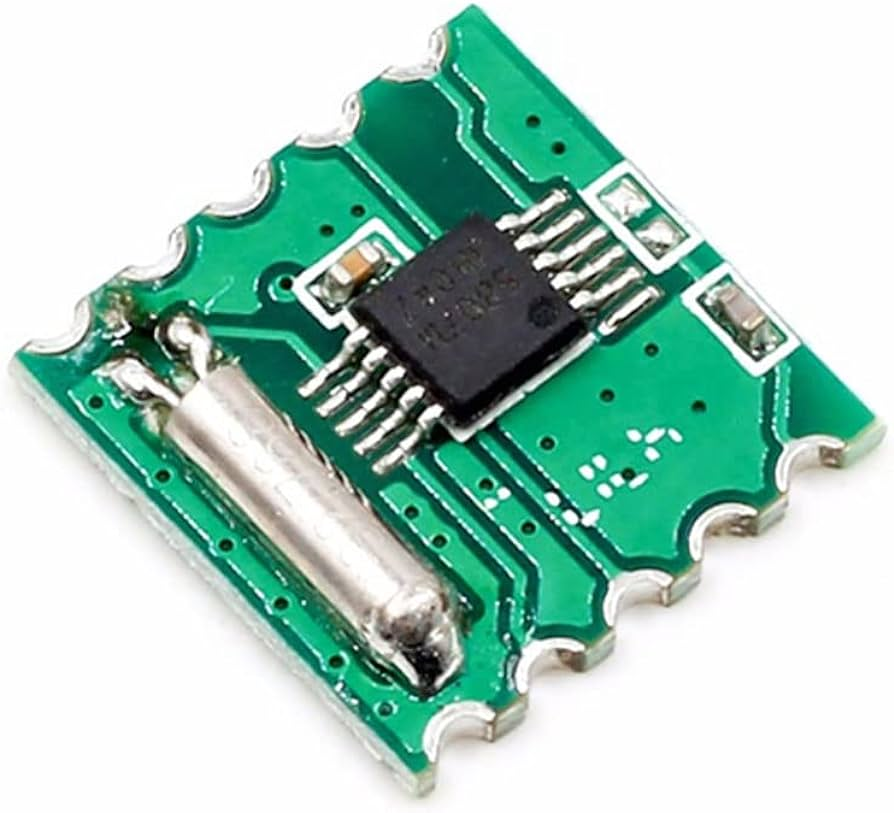
\includegraphics[width=0.3\textwidth]{images/2/2-3/Radio.jpg}
    \caption{Sintonizador FM RDA5807M}
    \label{fig:2-3-Radio}
\end{figure}
\subsection{Módulo MP3}
El modelo de MP3 seleccionado ha sido el YX5300, el cual se muestra en la \autoref{fig:2-3-MP3}.

Este reproductor se comunica con el microcontrolador mediante UART, con una velocidad de 9600 bps. También cuenta con una frecuencia de muestreo de 48 kHz y soporta tanto el formato MP3 como el formato WAV. Este modelo cuenta con un socket de tarjeta microSD en la cual se introducen las canciones, en los formatos antes mencionados, que se deseen reproducir. Dicha tarjeta deberá estar en formato Fat16 o Fat32 y tener como máximo \texttt{2 GB} de almacenamiento.

En cuento a la señal de audio obtenida a la salida del reproductor, podemos observar una salida bipolar entrada en 0V. Este comportamiento es totalmente inesperado ya que, al estar alimentado entre 3.3V y 0V, es extraño que la señal de salida pueda presentar valores negativos. Esto ha supuesto un gran problema en la unificación con el resto de módulos. Dicho problema y su solución será comentada en el \autoref{subsec:entre-dos-tierras}.

Por otra parte, el reproductor debe ser alimentadocon una tensión entre 3.2V y 5.2V, soporta una corriente máxima de 200mA y cuenta con un LED rojo que indica si está reproduciendo alguna canción.

Todas las características del reproductor MP3 se han obtenido del datasheet ofrecido por el fabricante. \cite{Catalex_MP3_boardPdf}

\begin{figure}[h]
    \centering
    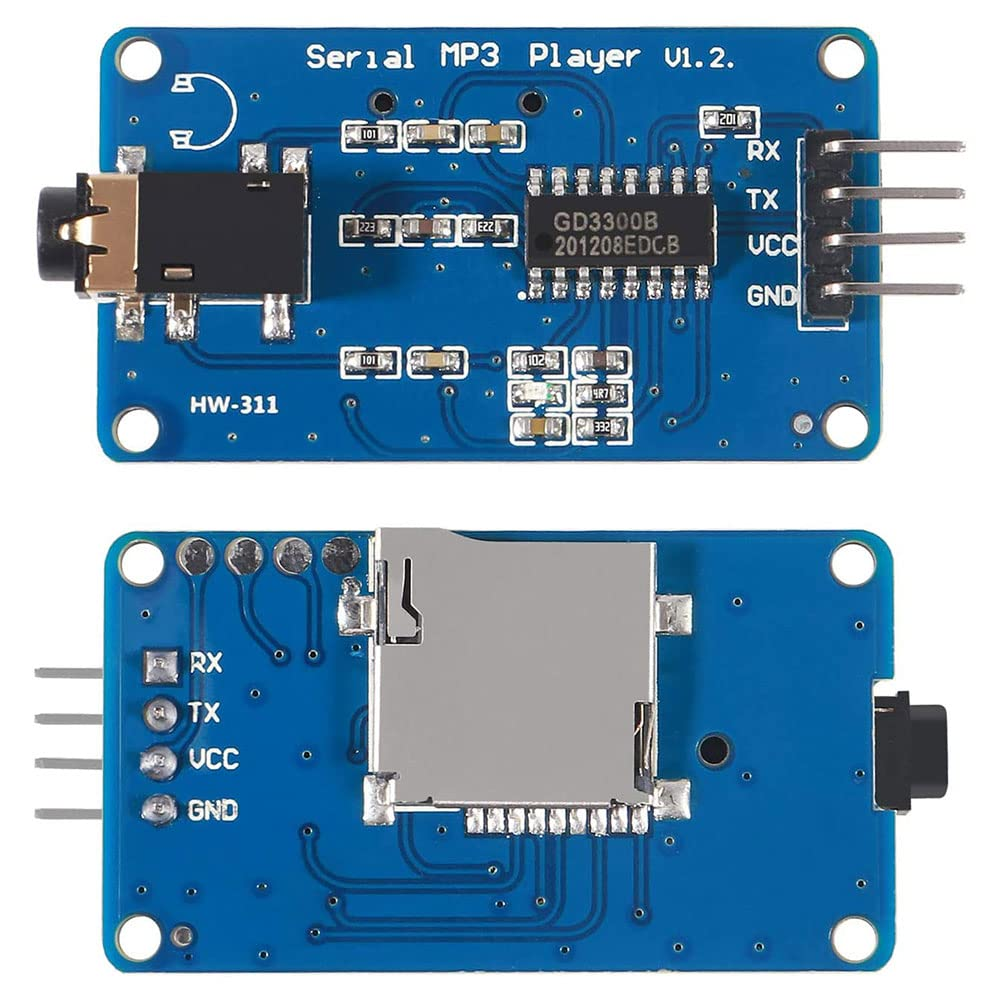
\includegraphics[width=0.3\textwidth]{images/2/2-4/MP3.jpg}
    \caption{Reproductor MP3 YX5300}
    \label{fig:2-3-MP3}
\end{figure}
\subsection{Módulo NFC}

Para su desarrollo, hemos utilizado el periférico I2C1, el protocolo RF, la placa \texttt{ANT7-T-M24SR64} \cite{M24SR64YPagWeb} de ST Microelectronics y la aplicación móvil \texttt{NFC Tools} \cite{NFCTools}. Además, a la hora de realizar comprobaciones desarrollando el módulo, hemos utilizado la app \texttt{ST25} \cite{ST25}.

\texttt{ANT7-T-M24SR64}: 
La placa \texttt{ANT7-T-M24SR64} es una placa que incluye un \texttt{M24SR64-Y}. \texttt{M24SR64-Y} es una tag dinámica NFC/RFID, EEPROM de interfaz dual, con protocolos RF e I2C. Se puede operar desde una interfaz I2C, un lector RFID o un teléfono con NFC.

\begin{figure}[h]
    \centering
    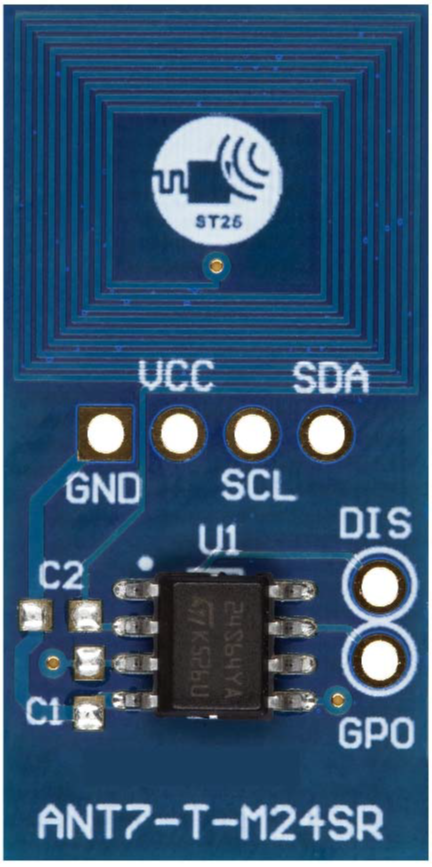
\includegraphics[width=0.15\textwidth]{images/2/2-5/M24SR.png}
    \caption{Módulo NFC \texttt{ANT7-T-M24SR64}}
    \label{fig:2-5-modulo-nfc}
\end{figure}

Como se puede observar en la figura anterior, hay 6 pines:

\begin{itemize}
    \item \texttt{VCC}: Alimentación 3.3 V.
    \item \texttt{GND}: Masa.
    \item \texttt{SDA}: Línea de datos del bus I2C.
    \item \texttt{SCL}: Señal de reloj del bus I2C.
    \item \texttt{GPO}: A nivel bajo, RF o I2C está siendo utilizado. A nivel alto, está libre.
    \item \texttt{DIS}: Activación/Desactivación de los comandos RF.
\end{itemize}

\subsection{Entre Dos Tierras}
\label{subsec:entre-dos-tierras}

El mayor problema al que nos hemos enfrentado en este proyecto es la gestión de las tierras en las señales de audio. Inicialmente diseñamos el circuito para que las señales de audio se conectaran entre la entrada de audio y la tierra virtual del circuito analógico, pensando que las señales serían compatibles con la entrada del ADC al estar alimentadas con los mismos niveles de tensión que los que las generan.

Sin embargo, descubrimos posteriormente que los circuitos compartían la tierra de audio de la entrada directamente con la salida, por lo que se realizaba un cortocircuito directo entre la tierra de la alimentación (o alimentación negativa visto desde el amplificador de audio) y la tierra virtual, por lo que se cortocircuitaban 3.5 V. 

Esto era claro en el lado del MP3 ya que el cortocircuito era a través de un camino de baja impedancia y provocaba que se activara la protección, desactivando la salida de audio. Sin embargo, debido a la circuitería interna o a las conexiones de la radio, había una pequeña pero no mínima impedancia que provocaba un consumo muy elevado de corriente pero que no llegaba al amperio, por lo que la protección no se disparaba. Esto es muy peligroso ya que es una potencia que se está disipando en el interior del chip y probablemente provoque daños si se mantiene el circuito en dicha condición.

Para solucionar este problema, decidimos construir unos cables de sonido en los cuales solo se conecte el terminal que lleva la señal, deshaciendo la conexión que realizan los sensores internamente.

Con estos ajustes la radio funcionaba bien, sin demasiado problema (excepto el ruido del que hablaremos a continuación). Sin embargo, el MP3 presenta otro problema. Contraintuitivamente, a pesar de estar alimentado con una tensión unipolar, el circuito del MP3 consigue generar una tensión bipolar simétrica con la señal de audio, señal completamente incompatible con nuestro sistema de muestreo con un ADC de la placa.

Para mediar este problema, hemos montado otro circuito analógico accesorio que mediante un divisor de tensión simétrico y un condensador de desacoplo consigue añadir una componente continua de 1.65 V a la tensión simétrica de entrada, haciendola completamente compatible con el sistema. Se añade una resistencia de \textit{Pull-down} en la entrada para evitar picos de tensión en el encendido del sistema. Los valores de las resistencias pueden ser cualesquiera valores grandes siempre que sean iguales y el condensador interesa elegirlo lo más grande posible. El circuito está recogido en la \autoref{fig:2-6-sumador}. 

\begin{figure}[h]
    \centering
    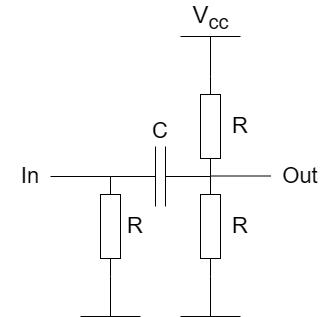
\includegraphics[width=0.5\textwidth]{images/2/2-6/sumadorEsquematico.png}
    \caption{Esquemático del circuito sumador}
    \label{fig:2-6-sumador}
\end{figure}

Se ha montado el circuito sobre una placa de baquelita, como se puede ver en la imagen de la \autoref{fig:2-6-foto-sumador}.\ 

\begin{figure}[h]
    \centering
    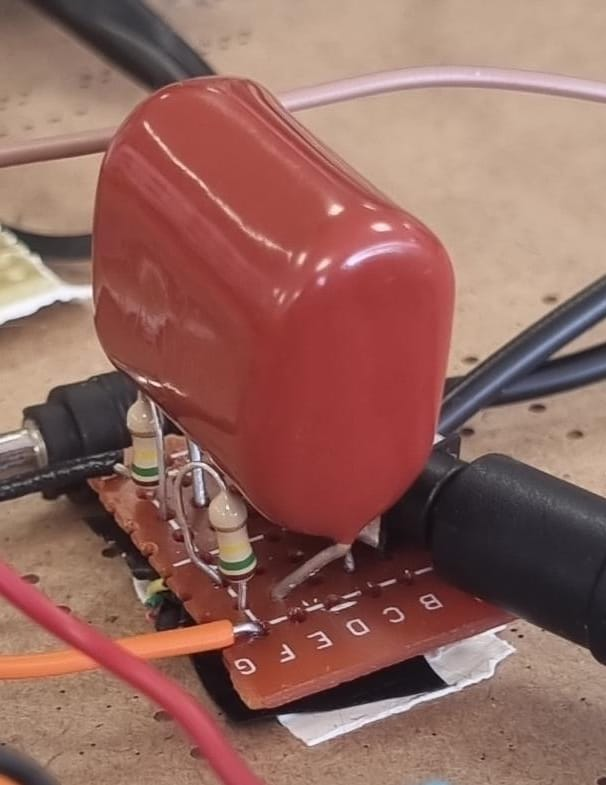
\includegraphics[width=0.25\textwidth]{images/2/2-6/fotoSumador.jpg}
    \caption{Foto del circuito sumador analógico}
    \label{fig:2-6-foto-sumador}
\end{figure}

Hemos elegido un valor de $100\ k\Omega$ para las resistencias y aproximadamente $1\ \mu F$ para el condensador, lo cual nos ofrece buenos resultados. Sin embargo, primero realizamos las pruebas con un condensador cerámico y no conseguimos que la tensión se estabilizara, por lo que se desplazaba el valor lentamente hacia uno de los raíles de alimentación. La solución que encontramos fue sustituirlo por un condensador de tántalo, que si bien tiene un tamaño físico considerablemente superior, consigue mantener de manera muy estable la tensión del circuito.

Este circuito funciona correctamente pero tiene la desventaja de decrementar ligeramente la tensión de entrada, provocando una caída en la relación señal-ruido del sistema.

Una vez solucionado el problema de las masas, aparece un ruido muy elevado en forma de zumbido y ruido blanco, por lo que el audio es de bastante baja relacion calidad ruido. Esto es principalmente debido a la longitud de los conductores por lo que va la señal, la cantidad de circuitos que atraviesa, etcétera. 

Además, la desconexión de las masas de los cables de audio provoca que el camino de retorno de las señales tenga que atravesar el resto del circuito y se deja de tratar la señal como un par diferencial, por lo que se pierde bastante calidad debido a la diferencia de tensión en las masas y algún posible bucle de masa al que se le acople algún ruido.

Por todo ello, si se quiere disfrutar de la máxima calidad de audio que puede ofrecer nuestro circuito, se debe desconectar la masa de la placa de la del circuito de amplificación de audio. El principal inconveniente de ello es que se deja de poder gestionar el multiplexor y la habilitación a través de los GPIO y no se puede realizar el procesado digital de señales.

Si se conectan los pines de selección y habilitación a los raíles de alimentación para seleccionar la configuración y se conecta un jumper entre los pines de ADC y DAC, se tiene una buenísima calidad de sonido, tanto en el altavoz como en los cascos. Se puede igualmente controlar la radio y el MP3 mediante las interfaces ya que eso no depende de la masa del circuito.

La mejor solución a este problema sería la realización de un circuito con alimentación simétrica verdadera. Esto se podría conseguir mediante dos baterías en serie (aunque sería un desperdicio ya que una solo se utilizaría para la parte negativa de la señal y no alimentaría la placa) o mediante la generación de una tensión negativa con un convertidor, por ejemplo, de tipo reductor-elevador con topología inversora. Igualmente se tendría que tener en cuenta la naturaleza bipolar de la señal del MP3 y se debería incluir el circuito de \textit{offset} a la placa o utilizar un cambiador de nivel analógico.
\subsection{Conexión de la alimentación a la placa}

Otro problema significativo que hemos encontrado es la conexión de la placa a la alimentación por baterías. La placa \texttt{STM32F769NI-Disco} indica que se puede alimentar con una tensión de entre 7 y 12 voltios en el pin de \texttt{Vin} siempre que se seleccione \texttt{ext5V} en los jumpers de selección de alimentación.

Probamos a alimentarlo con una fuente de tensión de laboratorio y el circuito funcionaba adecuadamente, consumiendo aproximadamente $300\ mA$. Sin embargo, al alimentarlo desde nuestro subsistema analógico, la placa funciona adecuadamente durante aproximadamente cinco segundos para después quedarse congelado. Hemos podido comprobar que es únicamente la CPU que se congela ya que las DMAs de audio siguen funcionando, reproduciendo el último contenido del buffer en bucle.

Hemos comprobado que no es un problema de tensión ya que, aunque en la hoja de catálogo indique que la placa requiere de mínimo 7 voltios, funciona bien incluso con $6.5\ V$ de la fuente de alimentación.

Tampoco es un problema de corriente ya que, como se explica en el apartado de test hardware, la placa puede aportar mucha más corriente que el aproximadamente medio amperio que requiere la placa.

% \section{Software}

\subsection{Interfaz de Usuario}
\subsubsection{Interfaz Web}
Para la visualización y representación de los distintos valores de tensión y corriente medidos por los diferentes sensores, se ha optado por utilizar ThingsBoard, una plataforma IoT de código abierto para la recopilación, el procesamiento, la visualización y la gestión de dispositivos de datos.

\begin{figure}[H]
    \centering
    
\includegraphics[width=0.3\textwidth]{images/3-software/3-2-2-thingsboard/LogoThingsboard.png}
    \caption{Plataforma ThingsBoard}
    \label{fig:3-2-2-ThingsBoard}
\end{figure}

Para su instalación en el ordenador, se ha optado utilizar una máquina virtual en VirtualBox mediante la imagen de un servidor Linux con distribución Ubuntu. Para la realización de dicha instalación se ha seguido la guía oficial de la plataforma de ThingsBoard, que se puede definir en los siguientes pasos: \cite{thingsboardInstallingThingsBoardCE}

\begin{enumerate}
    \item Instalar Java17 y configurarlo como predeterminado mediante los comandos:
    \begin{verbatim}
sudo apt update
sudo apt install openjdk-17-jdk
sudo update-alternatives --config java
    \end{verbatim}

    \item Instalar ThingsBoard mediante los siguientes comandos:
    \begin{verbatim}
wget https://github.com/thingsboard/thingsboard/releases/\
download/v3.8.1/thingsboard-3.8.1.deb
sudo dpkg -i thingsboard-3.8.1.deb
    \end{verbatim}

    \item Configurar la base de datos de ThingsBoard:
    \begin{verbatim}
sudo apt install -y postgresql-common
sudo /usr/share/postgresql-common/pgdg/apt.postgresql.org.sh
sudo apt -y install postgresql-16
sudo service postgresql start
sudo su - postgres
psql
    \end{verbatim}
    A continuación, elige tu contraseña del postgres mediante el siguiente comando:
    \begin{verbatim}
\password
    \end{verbatim}
    Después pulsa ``Ctrl + D'' para volver atrás y utiliza el siguiente comando para conectarte a la base de datos postgres:
    \begin{verbatim}
psql -U postgres -d postgres -h 127.0.0.1 -W
    \end{verbatim}
    Ahora, crea la base de datos para Thingsboard mediante el comando: \\
    \texttt{CREATE DATABASE thingsboard;} \\
    Por último, pulsa dos veces ``Ctrl + D'' para salir del PostgreSQL.

    \item Modificar el archivo de configuración de ThingsBoard mediante el siguiente comando:
    \begin{verbatim}
sudo nano /etc/thingsboard/conf/thingsboard.conf
    \end{verbatim}
    A continuación, añade estas líneas al final del archivo y no olvides cambiar \\
    \texttt{PUT\_YOUR\_POSTGRESQL\_PASSWORD\_HERE} por la contraseña del postgres que pusiste anteriormente:
    \begin{verbatim}
# DB Configuration
export DATABASE_TS_TYPE=sql
export SPRING_DATASOURCE_URL=jdbc:postgresql://localhost:5432/thingsboard
export SPRING_DATASOURCE_USERNAME=postgres
export SPRING_DATASOURCE_PASSWORD=PUT_YOUR_POSTGRESQL_PASSWORD_HERE
# Specify partitioning size for timestamp key-value storage.
# Allowed values: DAYS, MONTHS, YEARS, INDEFINITE.
export SQL_POSTGRES_TS_KV_PARTITIONING=MONTHS
    \end{verbatim}

    \item Elegir el tipo de servicio de cola de ThingsBoard. En este caso se elige el por defecto, en memoria, por lo que no es necesario ningún paso adicional.

    \item Ejecutar el script de instalación mediante el siguiente comando:
    \begin{verbatim}
sudo /usr/share/thingsboard/bin/install/install.sh --loadDemo
    \end{verbatim}

    \item Arrancar el servicio de ThingsBoard mediante el siguiente comando:
    \begin{verbatim}
sudo service thingsboard start
    \end{verbatim}
\end{enumerate}

Una vez realizados estos pasos, se podrá acceder a ThingsBoard mediante el siguiente link: \\
\url{http://localhost:8080/}

Por defecto, ThingsBoard incluye tres diferentes perfiles para acceder a la plataforma:
\begin{itemize}
    \item System Administrator: \texttt{sysadmin@thingsboard.org / sysadmin}
    \item Tenant Administrator: \texttt{tenant@thingsboard.org / tenant}
    \item Customer User: \texttt{customer@thingsboard.org / customer}
\end{itemize}

Debido al uso de la máquina virtual, se ha tenido que realizar una redirección de los puertos mediante la interfaz de red de la propia máquina, obteniendo la siguiente configuración:

\begin{figure}[H]
    \centering
    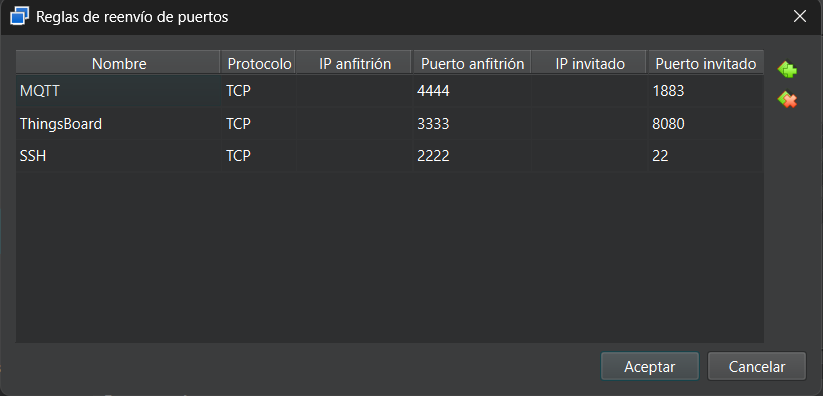
\includegraphics[width=0.3\textwidth]{images/3-software/3-2-2-thingsboard/PuertosMV.png}
    \caption{Redirección de puertos MV}
    \label{fig:3-2-2-PuertosMV}
\end{figure}

Por lo que, en nuestro caso, el puerto 1883 correspondiente al MQTT broker se corresponde con el puerto 4444 de la máquina virtual, el puerto 3333 de la plataforma ThingsBoard se corresponde con el puerto 8080 de la MV y también se ha redirigido el puerto 22 de SSH al puerto 2222 de la máquina virtual por conflictos internos con otro programa.

Para la comunicación entre la plataforma ThingsBoard y el dispositivo ESP8266, se ha implementado el broker Mosquitto, el cual es un broker MQTT OpenSource ampliamente utilizado debido a su ligereza, lo que permite fácilmente emplearlo en gran número de ambientes, incluso si éstos son de pocos recursos. A continuación se indica el comando necesario para su instalación, obtenido de la guía oficial de ThingsBoard: \cite{thingsboardMQTTDeviceAPI}

\begin{verbatim}
sudo apt-get install mosquitto-clients
\end{verbatim}

Para comprobar que todo se ha realizado correctamente, se puede utilizar el siguiente comando:
\begin{verbatim}
mosquitto_pub -d -q 1 -h "$THINGSBOARD_HOST_NAME" -p "1883"
-t "v1/devices/me/telemetry" -u "$ACCESS_TOKEN" -m {"ATTRIBUTE":25}
\end{verbatim}

Donde los siguientes parámetros corresponden con:
\begin{itemize}
    \item \texttt{THINGSBOARD\_HOST\_NAME}: dirección IP del servidor ThingsBoard, \\
    por ejemplo, \texttt{localhost} o \texttt{127.0.0.1}.
    \item \texttt{ACCESS\_TOKEN}: token de acceso único proporcionado por ThingsBoard para cada dispositivo.
    \item \texttt{ATTRIBUTE}: atributo asociado a dicho dispositivo, por ejemplo, temperature.
\end{itemize}

En caso de que la conexión y publicación se haya realizado de manera correcta, se obtendrá la siguiente respuesta:
\begin{verbatim}
Client mosqpub|xxx sending CONNECT
Client mosqpub|xxx received CONNACK
Client mosqpub|xxx sending PUBLISH
(d0, q1, r0, m1, 'v1/devices/me/telemetry', ... (16 bytes))
Client mosqpub|xxx received PUBACK (Mid: 1)
Client mosqpub|xxx sending DISCONNECT
\end{verbatim}

Una vez que se ha comprobado el correcto funcionamiento de la conexión entre la plataforma Thingsboard y el broker y cliente MQTT, se puede continuar con la personalización de dicha plataforma.

Para la visualización de los datos recibido, se ha optado por diseñar dos paneles o \textit{Dashboards}, uno en representación en forma de tablas y otro en forma de gráficas. Ambos paneles se actualizan en tiempo real y cuentan con una tabla o gráfica para cada dispositivo, obtenido un total de 4 tablas y 4 gráficas. Además, en las gráficas se puede visualizar también la media de los últimos datos medidos.

\begin{figure}[H]
    \centering
    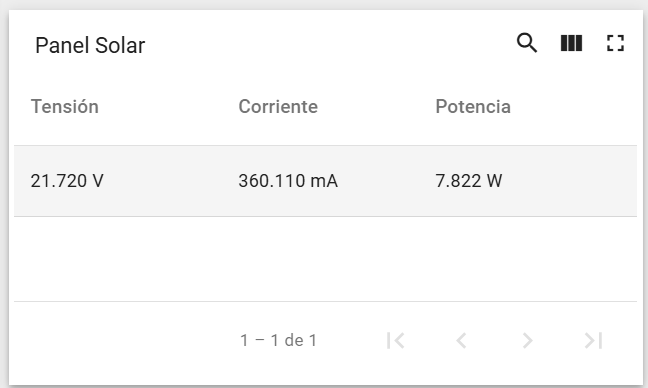
\includegraphics[width=0.3\textwidth]{images/3-software/3-2-2-thingsboard/TablaThingsBoard.png}
    \caption{Tabla de medidas}
    \label{fig:3-2-2-TablaThingsBoard}
\end{figure}

\begin{figure}[H]
    \centering
    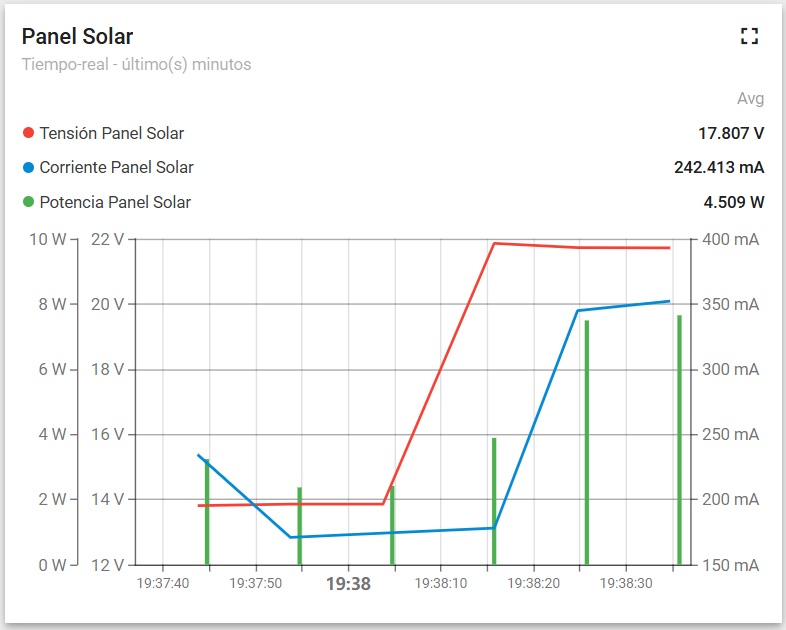
\includegraphics[width=0.3\textwidth]{images/3-software/3-2-2-thingsboard/GraficaThingsBoard.png}
    \caption{Gráfica de medidas}
    \label{fig:3-2-2-GraficaThingsBoard}
\end{figure}

Debido a que mediante los sensores solo se obtienen valores de tensión y de corriente, se ha implementado un algoritmo mediante las cadenas de reglas de Thingsboard. Se ha necesitado crear una cadena de reglas para cada potencia calculada, obteniendo 4 cadena de reglas como la siguiente:

\begin{figure}[H]
    \centering
    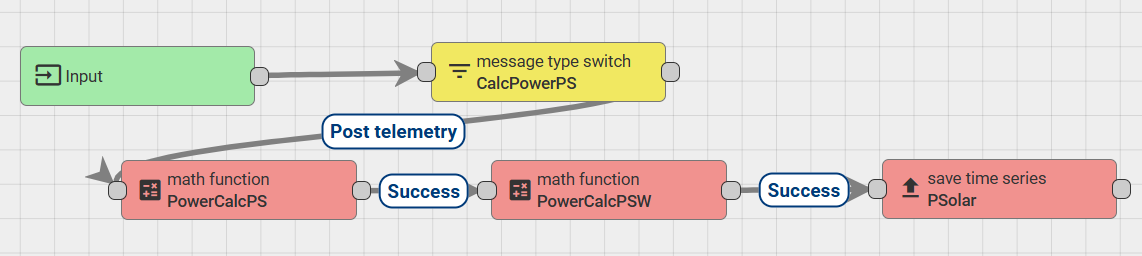
\includegraphics[width=0.3\textwidth]{images/3-software/3-2-2-thingsboard/CadenaPotencia.png}
    \caption{Cadena de reglas para cálculo de potencias}
    \label{fig:3-2-2-CadenaPotenciaThingsBoard}
\end{figure}

Dichas cadenas de reglas se dividen en los siguientes pasos:

\begin{enumerate}
    \item Filtrar y transformar la telemetría entrante
    \item Realizar el cálculo de la potencia correspondiente
    \item Pasar dicha potencia a Vatios
    \item Guardas los valores para su reprentación
\end{enumerate}

Por último, se ha añadido dichas cadenas de reglas de potencia a la cadena de regla principal, la cual gestiona el funcionamiento completo de Thingsboard y permite visualizar el dato obtenido de su respectiva cadena de regla.

\begin{figure}[H]
    \centering
    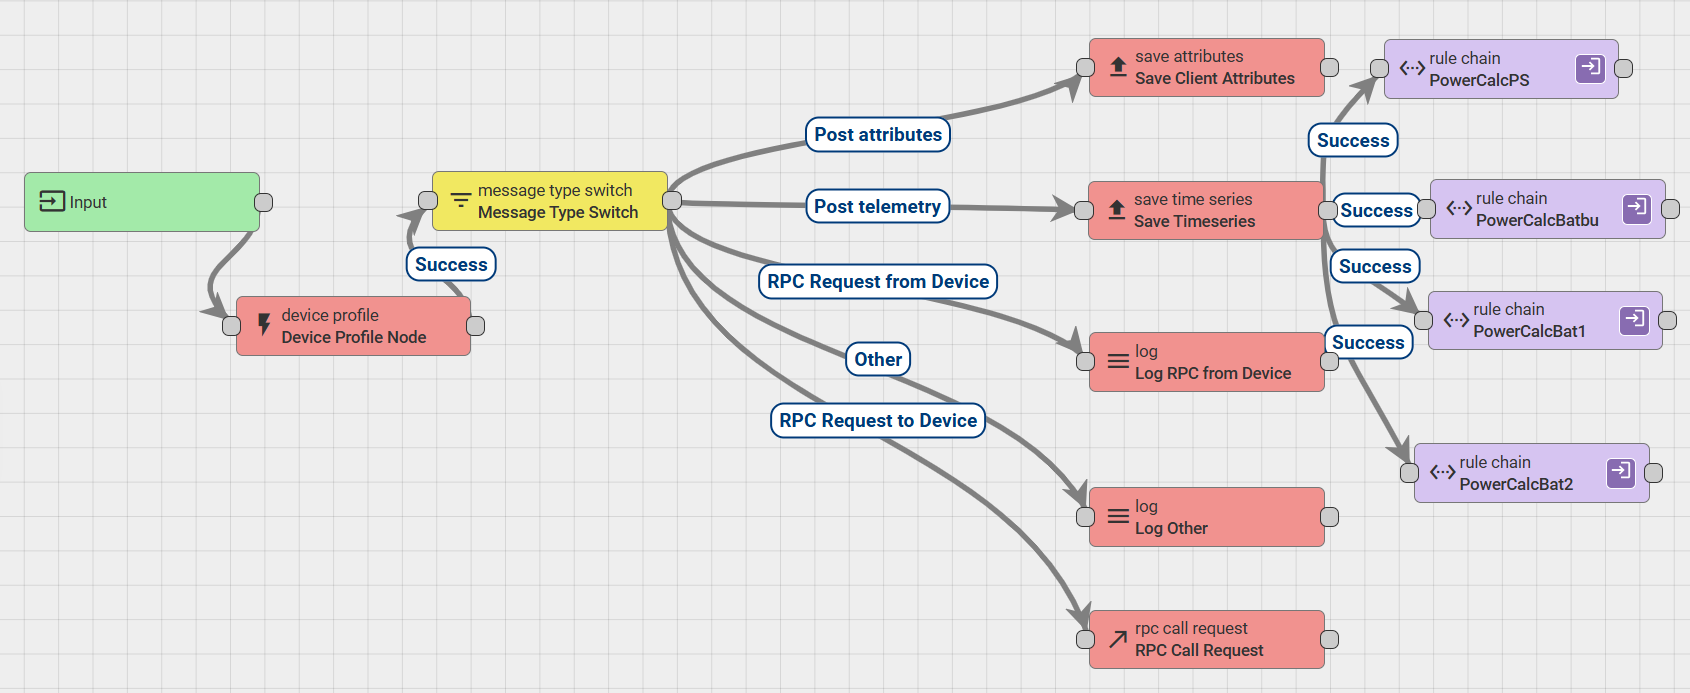
\includegraphics[width=0.3\textwidth]{images/3-software/3-2-2-thingsboard/CadenaPrincipal.png}
    \caption{Cadena de reglas principal}
    \label{fig:3-2-2-CadenaPrincipalThingsBoard}
\end{figure}

\subsection{Módulos Software}
\subsubsection{Módulo manejador de ficheros}\label{subsubsec:ManejadorFicheros}
El módulo de gestión de fichero es el encargado de realizar tanto la escritura, lectura o eliminación del fichero que almacena las medidas obtenidas. Esta formado por dos archivos, \texttt{file\_management.cpp} el cual contiene las funciones necesarias, y \texttt{file\_management.hpp}, el cual contiene la definición de las funciones y la importación de la librería externa utilizada.


Para la implementación de este módulo se ha requerido la utilización de \texttt{SPIFFS} incluido en la librería externa \texttt{FS}. \texttt{SPIFFS} o \texttt{SPI Flash File System} es un sistema de archivos diseñado para funcionar en memorias flash conectadas por \texttt{SPI}, lo que lo hace perfecto para este proyecto.

\begin{figure}[H]
    \centering
    
\includegraphics[width=0.3\textwidth]{images/3-software/3-2-1-filemng/esp8266-spiffs.png}
    \caption{\texttt{SPIFFS}}
    \label{fig:3-2-1-1-SPIFFS}
\end{figure}

El fichero \texttt{file\_management.cpp} consta de las tres siguientes funciones:
\begin{itemize}
    \item \texttt{Clear\_file}: esta función se encarga de borrar el fichero. Recibe como parámetro el fichero a borrar y no devuelve nada. La secuencia de ejecución es la siguiente:
    \begin{enumerate}
        \item Inicializa el \texttt{SPIFFS}.
        \item Abre el fichero en modo escritura.
        \item Cierra el archivo.
    \end{enumerate}
    Al abrir el fichero en modo escritura y no escribir nada, el archivo queda borrado.
    \begin{lstlisting}[captionpos=b, caption={Funcion \texttt{Clear\_file}}, language=c++]
void clear_file(const char* measFile) {
    if (!SPIFFS.begin()) {
        Serial.println("[FILE_MGT] Error iniciando SPIFFS");
        return;
    }

    File file = SPIFFS.open(measFile, "w");
    if (!file) {
        Serial.println("[FILE_MGT] Error abriendo el fichero para borrar");
        return;
    }

    file.close();
    Serial.println("[FILE_MGT] El contenido del fichero ha sido borrado.");
}
    \end{lstlisting}
    \item \texttt{Read\_meas}: esta función realiza la operación de lectura del fichero. Recibe como parámetro el fichero a leer y no devuelve nada. La secuencia de ejecución es la siguiente:
    \begin{enumerate}
        \item Inicia el \texttt{SPIFFS}.
        \item Abre el fichero en modo de lectura.
        \item Muestra por \texttt{Serial} el contenido del archivo hasta que detecta que acaba dicho fichero.
        \item Cierra el fichero.
    \end{enumerate}
    \begin{lstlisting}[captionpos=b, caption={Funcion \texttt{Read\_file}}, language=c++]
void read_meas(const char* measFile){
    if (!SPIFFS.begin()) {
        Serial.println("[FILE_MGT] Error iniciando SPIFFS");
        return;
    }

    File measurementFile = SPIFFS.open(measFile, "r");
    if (!measurementFile) {
        Serial.println("[FILE_MGT] Error abriendo fichero");
        return;
    }

    Serial.println("[FILE_MGT] Abriendo " + String(measFile) + ". Contenido: ");

    while (measurementFile.available()) {
        Serial.write(measurementFile.read());
    }

    measurementFile.close();
}
    \end{lstlisting}
    \item \texttt{Write\_meas}: esta función realiza la operación de escritura en el fichero. Recibe como parámetros el fichero a escribir, las medidas obtenidas por los sensores y una cadena de texto con la fecha y hora en la cual se han realizado dichas medidas y devuelve un  booleano que indica si la operación se ha realizado de manera correcta. La secuencia de ejecución es la siguiente:
    \begin{enumerate}
        \item Inicia el \texttt{SPIFFS}.
        \item Abre el fichero en modo \texttt{append} para escribir a continuación de la última medida y no sobrescribirla.
        \item Se forma la cadena de texto que se desea escribir. Dicha cadena está formada por la fecha y hora de la medición y por los valores obtenidos.
        \item Se escribe dicha cadena en el fichero.
        \item Se cierra el fichero.
        \item En caso de que la escritura haya sido satisfactoria, esta función devolverá true, en caso de que se haya encontrado un error en cualquiera de los pasos realizados, esta función devolverá false.
    \end{enumerate}
    \begin{lstlisting}[captionpos=b, caption={Funcion \texttt{Write\_file}}, language=c++]
bool write_meas(const char* measFile, telemetry_t measures, String timestamp) {
    if (!SPIFFS.begin()) {
        return false;
    }

    File measurementFile = SPIFFS.open(measFile, "a");
    if (!measurementFile) {
        return false;
    }

    String measurement = timestamp +
                            " VPanelSolar: " + String(measures.VSolar) + " V, " +
                            "IPanelSolar: " + String(measures.ISolar) + " mA, " +
                            "VBatBackup: " + String(measures.VBatbu) + " V, " +
                            "IBatBackup: " + String(measures.IBatbu) + " mA, " +
                            "VBat1: " + String(measures.VBat1) + " V, " +
                            "IBat1: " + String(measures.IBat1) + " mA, " +
                            "VBat2: " + String(measures.VBat2) + " V, " +
                            "IBat2: " + String(measures.IBat2) + " mA";

    measurementFile.println(measurement);
    measurementFile.close();

    return true;
}
    \end{lstlisting}
\end{itemize}

\subsubsection{Fichero Hardware.h}

El fichero "Hardware.h" define los pines que utiliza el ESP. 

Siendo estos pines:
\begin{itemize}
    \item \textbf{PIN13 y PIN15}: Para la gestión de la conmutación de los relés. 
    \item \textbf{PIN4 y PIN5}: Usados para la gestión de la comunicación I2C (Señales SDA y SCL respectivametne). 
\end{itemize}


\subsubsection{Modulo INA}

El módulo INA es el encargado de realizar la configuración de los INAs y solicitarles medidas.
Este módulo está formado por dos archivos:
\begin{itemize}
    \item ina.cpp : Contiene las funciones necesarias para la configuración de los sensores, el bajo consumo y la toma de medidas.
    \item ina.hpp : Contiene la definición de la función que solicita 1 única medida a los INA y las direcciones I2C de los INA.
\end{itemize}

Para la implementación de este módulo se ha requerido la utilización de la librería \texttt{"INA266\_WE.h"} ,que permite configurar y leer los datos mediante I2C con Arduino.
%\TODO{ https://github.com/wollewald/INA226_WE}

El fichero ina.cpp contiene las siguientes funciones:

- \texttt{setupINA226Sensors()}: Esta función inicializa los 4 INAs con la configuración inicial que establece la librería \texttt{“INA266\_WE.h”}.

\begin{lstlisting}[captionpos=b, caption={Codigo funcion setupINA226Sensors}, language=c++]
    void setupINA226Sensors() {
        Wire.begin();
        Solar.init();
        Batbu.init();
        Bat1.init();
        Bat2.init();
    }
\end{lstlisting}

- \texttt{reconfig\_INAs()}: Al despertar o inicializarlos INA, se encuentran con la configuración por defecto, por lo que es necesario reconfigurarlos acorde a las necesidades de nuestro circuito. Esta reconfiguración consta de lo siguiente:
\begin{itemize}
    \item \texttt{setConversionTime}: Establece el tiempo que asignamos al INA para realizar la conversión de medidas físicas a su valor digital.
    \item \texttt{setMeasureMode}: Establece el modo de medida, POWER\_DOWN (Sistema apagado), TRIGGERED (medidas a petición) o CONTINUOUS (medidas constantes).
    \item \texttt{setResistorRange}: Establece el valor de la resistencia de SHUNT que tiene el INA (Medido físicamente) y su rango de corriente con el que se va a trabajar.
    \item \texttt{setCorrectionFactor}: Establece el factor de corrección, el sensor nunca realiza una medición que corresponde con la realidad, por lo que es necesario indicar el factor de corrección que tiene que ser aplicado cuando se realizan estas medidas. Para el establecimiento de este valor se han realizado medidas experimentales midiendo el valor real y comparándolo con lo que indicado por el sensor.
\end{itemize}


\begin{lstlisting}[captionpos=b, caption={Codigo funcion reconfig\_INAs}, language=c++]
    void reconfig_INAs(){
        Solar.setConversionTime(CONV_TIME_1100);
        Batbu.setConversionTime(CONV_TIME_1100);
        Bat1.setConversionTime(CONV_TIME_1100);
        Bat2.setConversionTime(CONV_TIME_1100);
    
        Solar.setMeasureMode(CONTINUOUS);
        Batbu.setMeasureMode(CONTINUOUS);
        Bat1.setMeasureMode(CONTINUOUS);
        Bat2.setMeasureMode(CONTINUOUS);
        
        Solar.setResistorRange(0.1, 10);
        Batbu.setResistorRange(0.1, 10);
        Bat1.setResistorRange(0.1, 10);
        Bat2.setResistorRange(0.1, 10);
        
        // Factores de correccion medidos experimentalmente
        Solar.setCorrectionFactor(1.0469);
        Batbu.setCorrectionFactor(1.0419);
        Bat1.setCorrectionFactor(0.9650);
        Bat2.setCorrectionFactor(0.9624);
        
        Solar.waitUntilConversionCompleted();
        Batbu.waitUntilConversionCompleted();
        Bat1.waitUntilConversionCompleted();
        Bat2.waitUntilConversionCompleted();
    }
\end{lstlisting}

- \texttt{powerDownINA226()}: Pone en bajo consumo los INA ya que tras conseguir las medidas no es necesario que se mantengan activos.

\begin{lstlisting}[captionpos=b, caption={Codigo funcion powerDownINA226}, language=c++]
    void powerDownINA226() {
        Solar.powerDown();
        Batbu.powerDown();
        Bat1.powerDown();
        Bat2.powerDown();
    }
\end{lstlisting}


- \texttt{powerUpINA226()}: Despierta de nuevo a los INA, al despertarlos los sensores se reinician con la configuración por defecto por lo que es necesario reconfigurarlos.

\begin{lstlisting}[captionpos=b, caption={Codigo funcion powerUpINA226}, language=c++]
    void powerUpINA226() {
        Solar.powerUp();
        Batbu.powerUp();
        Bat1.powerUp();
        Bat2.powerUp();
    }
\end{lstlisting}

-\texttt{measureINA226(telemetry\_t *telemetry)}: Realiza la medida de todos los sensores. La secuencia de ejecución es la siguiente:

\begin{enumerate}
    \item Verifica si se han inicializado 1 vez los INAs. Si se han inicializado se despiertan.
    \item Se reconfiguran.
    \item Se toman las medidas de tensión y corriente de todos los INAs y se guarda la información en el puntero con la estructura de datos.
    \item Se ponen a bajo consumo los INAs.
\end{enumerate}

\begin{lstlisting}[captionpos=b, caption={Codigo funcion measureINA226}, language=c++]
    void measureINA226(telemetry_t *telemetry) {
        // Panel Solar
        if(first_config==false){
          setupINA226Sensors();
          first_config=true;
        }else{
          powerUpINA226();  
        }
    
        reconfig_INAs();
        
        Solar.readAndClearFlags();
        telemetry->VSolar = Solar.getBusVoltage_V() + (Solar.getShuntVoltage_mV() / 100);
        telemetry->ISolar = Solar.getCurrent_mA();
    
        // Bateria Backup
        Batbu.readAndClearFlags();
        telemetry->VBatbu = Batbu.getBusVoltage_V() + (Batbu.getShuntVoltage_mV() / 100);
        telemetry->IBatbu = -Batbu.getCurrent_mA();
    
        // Bateria 1
        Bat1.readAndClearFlags();
        telemetry->VBat1 = Bat1.getBusVoltage_V() + (Bat1.getShuntVoltage_mV() / 100);
        telemetry->IBat1 = -Bat1.getCurrent_mA(); // Invertir signo porque esta al reves
    
        // Bateria 2
        Bat2.readAndClearFlags();
        telemetry->VBat2 = Bat2.getBusVoltage_V() + (Bat2.getShuntVoltage_mV() / 100);
        telemetry->IBat2 = Bat2.getCurrent_mA();
        powerDownINA226();
    }
\end{lstlisting}


En el contenido de este mismo fichero, se instancian los 4 INAs que tenemos indicando su dirección I2C:

\begin{lstlisting}[captionpos=b, caption={Instancia de las direcciones de los INAs.}, language=c++]
    #include "ina.hpp"
    // INA226 instances
    INA226_WE Solar(I2C_D_PANEL);
    INA226_WE Batbu(I2C_D_BAT_BU);
    INA226_WE Bat1(I2C_D_BAT_1);
    INA226_WE Bat2(I2C_D_BAT_2);
    
\end{lstlisting}



\subsubsection{Modulo Cliente MQTT}

El módulo MQTT es el encargado de crear un cliente MQTT y establecer una conexión con el servidor MQTT para enviar los datos de la ultima medida que se haya realizado. 

Este módulo está formado por dos archivos:
\begin{itemize}
    \item \texttt{mqtt\_client.cpp} : Contiene las funciones necesarias para la conexión.
    \item \texttt{mqtt\_client.hpp} : Contiene la definición de las funciones, la importación de las librerías externas utilizadas y el número de reintentos permitidos al realizar una conexión con el servidor.
\end{itemize}

Para la implementación de este módulo se ha requerido la utilización de las librerías \texttt{“PubSubClient.h”}, que permite la conexión MQTT, \texttt{“ESP8266WiFi.h”} y \texttt{“WiFiUdp.h”} para configurar el cliente UDP.\cite{olearyKnollearyPubsubclient2024}

El fichero \texttt{mqtt\_client.cpp} contiene las siguientes funciones:

-\texttt{reconnect(PubSubClient\& client, char* const mqtt\_server, int mqtt\_port)}: Para intentar una reconexión con el servidor MQTT en caso de que haya fallado. Aunque este intento de reconexión es limitando.

-\texttt{bool publishTelemetry(char* const mqtt\_server, int mqtt\_port, telemetry\_t\& telemetry)}: Intenta publicar un mensaje con todos los datos medidos por el INA al servidor MQTT.  La secuencia de ejecución es la siguiente:
\begin{enumerate}
    \item Crea un cliente MQTT.
    \item Crea una conexión con el servidor MQTT.
    \item Verifica si el cliente se ha podido conectar con el servidor. Si no ha podido intenta realizar una reconexión en el caso de que haya habido un error.
    \item Formatea el mensaje para que pueda ser procesado por el servidor.
    \item Publica el mensaje en el servidor y este devuelve un booleano que indica si el envío ha sido correcto.
    \item Se desconecta el cliente.
    \item Devuelve el booleano.
\end{enumerate}


\subsubsection{Módulo Bajo Consumo}
El módulo de bajo consumo es el encargado de reducir el consumo del sistema cuando no es necesario que funcione a plena potencia, es decir, entre las obtenciones de las diferentes medidas.

Las librerías incluidas con el \texttt{ESP8266} incluye un modo de bajo consumo ya definido llamado \texttt{deep-sleep}, el cual desactiva el \texttt{WiFi}, el reloj del sistema y la \texttt{CPU}, es decir, solo mantiene el funcionamiento del \texttt{RTC} y reduce el consumo del sistema a apenas unas decenas de microamperios. Sin embargo, debido a que este modo de bajo consumo inhabilita también los \texttt{GPIO} es incompatible con nuestro sistema, ya que si se activara, el sistema no sería capaz de mantener los relés conmutados al entrar a este modo. Debido a esto, este modo de bajo consumo no es apto para nuestro sistema. \cite{esp8266ESP8266LowPower}

\begin{figure}[H]
    \centering
    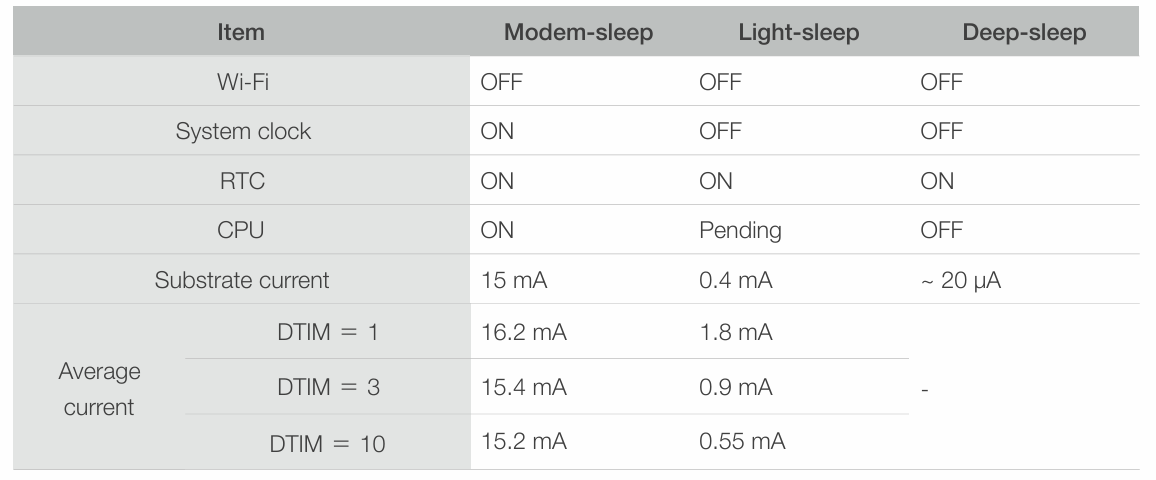
\includegraphics[width=0.6\textwidth]{images/3-software/3-2-5-lowpower/Modos Bajo Consumo.png}
    \caption{Modos Bajo Consumo ESP8266}
    \label{fig:3-2-5-1-ModosBajoConsumo}
\end{figure}

Debido a este requisito, hemos desarrollado nuestro propio modo de bajo consumo, el cual reduce el consumo del sistema en un $80\%$ aproximadamente. Este modo de bajo consumo es similar al llamado modem-sleep. Por nuestra parte, nuestro modo desactiva el wifi, baja la frecuencia del reloj del sistema y ejecuta un \texttt{delay}, para que el micro reduzca su consumo. Debido a que en ningún momento se inhabilitan los \texttt{GPIO}, este modo de bajo consumo es perfecto para nuestro sistema.

Este módulo esta dividido en dos ficheros, \texttt{sleep.hpp} el cual contiene la definición de la función de bajo consumo y la importación de la librería necesaria, y el fichero \texttt{sleep.cpp}, el cual contiene la implementación de dicha función, que recibe como parámetro el tiempo en milisegundos deseado de duración del modo de bajo consumo y no devuelve nada.

\begin{lstlisting}[captionpos=b, caption={Función bajo consumo}, language=c++]
    void sleep_low_power(int time_delay) {}
\end{lstlisting}

La secuencia de ejecución se puede dividir en dos secuencias consecutivas, una que activa el modo de bajo consumo y otra que restaura el funcionamiento normal. La secuencia de activación es la siguiente:

\begin{enumerate}
    \item Se desactiva el módulo de \texttt{WiFi}, activando el modo \texttt{WIFI\_OFF}.
    \item Se llama a la función \texttt{forceSleepBegin()}, la cual guarda el modo de \texttt{WiFi} actual y fuerza el estado de modo \texttt{sleep} del \texttt{WiFi}, reduciendo aún más el consumo.
    \item Se reduce la frecuencia del reloj del sistema al mínimo valor posible, $80\ MHZ$.
    \item Se introduce un \texttt{delay}. Esto asegura que el microprocesador consumirá menos durante dicho tiempo, además se utiliza para definir la duración aproximada del modo de bajo consumo.
\end{enumerate}

\begin{lstlisting}[captionpos=b, caption={Activación modo bajo consumo}, language=c++]
Serial.println("[SLEEP] Entrando en modo bajo consumo");
WiFi.mode(WIFI_OFF);
WiFi.forceSleepBegin();
system_update_cpu_freq(SYS_CPU_80MHZ);

delay(time_delay);
\end{lstlisting}

Una vez pasado el tiempo definido de bajo consumo, se entra en la secuencia de restauración, la cual consta de los siguientes pasos:

\begin{enumerate}
    \item Aumentar la frecuencia del reloj al valor anterior, 160 MHz.
    \item Forzar la activación del módulo del \texttt{WiFi}.
    \item Aplicar un \texttt{delay} de $1\ ms$ para asegurar que el módulo \texttt{WiFi} se haya despertado.
    \item Configurar el módulo de \texttt{WiFi} como una estación, es decir, configurar el \texttt{ESP8266} como un dispositivo que se conecta a un punto de acceso.
\end{enumerate}

\begin{lstlisting}[captionpos=b, caption={Restauración modo bajo consumo}, language=c++]
Serial.println("[SLEEP] Saliendo del modo bajo consumo");
system_update_cpu_freq(SYS_CPU_160MHZ);
WiFi.forceSleepWake();
delay(1);
WiFi.mode(WIFI_STA);
\end{lstlisting}

Mediante la implementación de nuestro propio modo de bajo consumo, nos aseguramos que correcto funcionamiento durante y después de dicho modo, reduciendo el consumo del sistema un 80\% aproximadamente, pasando de un consumo de 73 mA aporximadamente a pleno funcionamiento, a apenas 15 mA en el estado de bajo consumo.


\subsubsection{Módulo Telemetría}

El fichero \texttt{telemetry.hpp} define la estructura de datos que usaremos para la telemetría.

Dicha estructura almacenará los datos de las medidas obtenidas por los \texttt{INA}, es decir, los datos de tensión y corriente de las baterías (del usuario y \textit{Backup}) y del panel solar.

\begin{lstlisting}[language=c++,caption={Estructura de datos para la telemetría},captionpos=b]
typedef struct {
    float VSolar;  /** Tension panel solar      */
    float ISolar;  /** Corriente panel solar    */
    float VBatbu;  /** Tension bateria backup   */
    float IBatbu;  /** Corriente bateria backup */
    float VBat1;   /** Tension bateria 1        */
    float IBat1;   /** Corriente bateria 1      */
    float VBat2;   /** Tension bateria 2        */
    float IBat2;   /** Corriente bateria 2      */
} telemetry_t;
\end{lstlisting}

\subsection{Programa Principal}
\documentclass{article}
\begin{document}
\subsection{Modulo Principal}

Este módulo está formado por el archivo, \texttt{MAIN\_POWER.ino} que se encarga de conectar todos los módulos en un sistema unificado.

El fichero contiene las siguientes funciones:

- \texttt{setup()}: Inicializa los pines que usamos para la comunicación I2C y los relés, la velocidad del puerto serie y el valor inicial de la estructura de datos que contienen.

- \texttt{loop()}: Realiza todas las operaciones de funcionamiento del sistema. La secuencia de ejecución es la siguiente:
\begin{enumerate}
    \item Recoge las medidas de losz INA.
    \item Revisa los valores obtenidos del panel solar por si es necesario cambiar la alimentación del panel solar a la de backup.
    \item Se intenta conectar a la red Wifi. Si lo consigue se intenta mandar las medidas al servidor mqtt.
    \item Guarda las medidas de los sensores en un fichero.
    \item Duerme al ESP poniéndolo en bajo consumo.
    \item Sale del modo de bajo consumo.
\end{enumerate}

\end{document}


\subsection{Programa Lectura Fichero}
Para la lectura del fichero almacenado en la memoria \texttt{FLASH} del dispositivo, el cual contiene las medidas obtenidas por los sensores, se ha desarrollado un programa independiente el cual se encarga de realizar esta función. Además, permite la eliminación de dicho fichero. Para ejecutar dichas funciones, se enviará por serial al micro un caracter u otro mediante el teclado. Ambas operaciones se realizan mediante el sistema de archivos \texttt{SPIFFS}.


Para la realización de este programa, se ha utilizado las funciones \texttt{Clear\_file} y \texttt{Read\_meas} explicadas en el \autoref{subsubsec:ManejadorFicheros}, por lo que ha sido necesario importar el archivo \texttt{file\_management.hpp}, el cual contiene las definiciones de dichas funciones.

Este programa se puede dividir en dos partes, la función \texttt{setup()}, la cual se ejecuta tan solo una vez al arrancar el programa, y la función \texttt{loop()}, la cual consiste en un bucle infinito con el principal funcionamiento del programa. A continuación, se va a explicar el funcionamiento de estas dos funciones:

\begin{itemize}
    \item \textbf{\texttt{setup()}:} Esta función tan solo inicializa el serial a una velocidad de \texttt{9600 bps}, y muestra el siguiente mensaje por serial al usuario:
    \begin{figure}[H]
        \centering
        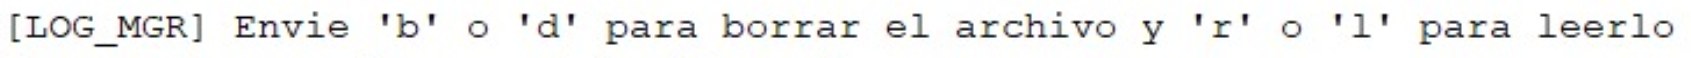
\includegraphics[width=0.8\textwidth]{images/3-software/3-4-readfile/MensajeInicial.png}
        \caption{Mensaje inicial programa de lectura}
        \label{fig:3-4-1-MensajeInicial}
    \end{figure}
    \item \textbf{\texttt{loop()}:} Contiene el principal funcionamiento del programa y su secuencia de ejecución es la siguiente:
    \begin{enumerate}
        \item Verificar si el serial funciona correctamente. En caso de que el serial no esté en pleno funcionamiento, el programa no hace nada.
        \item Lee el caracter enviado mediante el serial y lo guarda en una variable.
        \item En caso de que dicho caracter sea una \texttt{b} o una \texttt{d}, se procede a la secuencia de eliminación del fichero. Dicha secuencia es la siguiente:
        \begin{enumerate}
            \item Se muestra por serial un mensaje indicando al usuario la acción realizada.
            \item Se llama a la función \texttt{clear\_file}, incluida en la librería \texttt{file\_management.hpp}, pasándole como parámetro el archivo a eliminar.
            \item Una vez eliminado el fichero, se realiza una comprobación de la existencia de dicho archivo, mostrando por serial el estado del archivo.
            \item Se cierra el archivo.
        \end{enumerate}
        \item Por otra parte, en caso de que el caracter leído haya sido una 'r' o una 'l', se procede a la lectura del fichero, llamando a la función \texttt{read\_meas}, en la librería \texttt{file\_management.hpp}, pasándole como parámetro el archivo a leer.
        \item En caso de que el caracter no haya sido ninguno de los anteriores mencionados, el sistema mostrará por serial el mismo mensaje que al principio de la ejecución de este programa, indicando al usuario que caracteres son aceptados.
    \end{enumerate}
    \begin{lstlisting}[captionpos=b, caption={Programa lectura o eliminación de fichero}, language=c++]
        #include "file_management.hpp"

        const char* testFile = "/measurements.txt";

        void setup() {
          Serial.begin(9600);
          Serial.println("[LOG_MGR] Envie 'b' o 'd' para borrar el archivo y 'r' o 'l' para leerlo ");
        }

        void loop() {
            // Verificar si hay datos disponibles en el puerto serial
            if (Serial.available() > 0) {
                char command = Serial.read(); // Leer el caracter ingresado
                if (command == 'b' ||  command == 'd') {

                    Serial.println("[LOG_MGR]Borrando contenido del archivo...");
                    clear_file(testFile);

                    // Confirmar estado del archivo despues de borrarlo
                    File file = SPIFFS.open(testFile, "r");
                    if (file && file.available()) {
                        Serial.println("[LOG_MGR] El archivo aun tiene contenido.");
                    } else {
                        Serial.println("[LOG_MGR] El archivo esta vacio.");
                    }
                    file.close();
                } else if (command == 'r' ||  command == 'l') {
                    read_meas(testFile);
                } else if (command != '\n') {
                  Serial.println("[LOG_MGR] Envie 'b' o 'd' para borrar el archivo y 'r' o 'l' para leerlo ");
                }
            }
        }
    \end{lstlisting}
\end{itemize}



\subsection{Librerías Externas}
\subsubsection{Librería INA}
Una de las librerías utilizadas para realizar el proyecto ha sido la librería \texttt{INA226\_WE}.  Esta contiene toda la información necesaria para la comunicación \texttt{I2C}, configuración y obtención de datos de los sensores \texttt{INA226}, además de otras herramientas útiles como el establecimiento del modo de bajo consumo para los sensores.

En nuestro proyecto hemos utilizado esta herramienta para obtener los datos de tensión y corriente de los 4 \texttt{INAs}.  Aunque adicionalmente, se han utilizado las herramientas de configuración para ajustar de manera correcta los sensores y que estas medidas obtenidas sean fieles a la realidad, además de utilizar su modo de bajo consumo cuando no era necesario obtener medidas.

La versión utilizada es la \texttt{1.2.9} y pueden obtenerse los ficheros fuente en su repositorio en \texttt{GitHub}. \cite{ewaldWollewaldINA226_WE2024}

Adicionalmente, se cuenta con una página con documentación completa de esta librería y su funcionamiento. \cite{ewaldINA226CurrentPower2021}

\subsubsection{Librería PubSubClient}
La librería utilizada para implementar el cliente \texttt{MQTT} ha sido la librería \texttt{PubSubClient}.  Esta contiene toda la información necesaria para la creación de un cliente \texttt{MQTT}, la conexión con un servidor \texttt{MQTT} y la publicación y recepción de mensajes de servidores \texttt{MQTT}.

En nuestro proyecto hemos utilizado esta herramienta únicamente para la conexión con el servidor \texttt{MQTT} y el envío de los datos de las medidas de los \texttt{INA}.

La versión utilizada es la \texttt{2.8} y pueden obtenerse los ficheros fuente en su repositorio en \texttt{GitHub}. \cite{olearyKnollearyPubsubclient2024}

Adicionalmente, se cuenta con una página con documentación completa de esta librería y su funcionamiento. \cite{nickolearyArduinoClientMQTT}

\todo[inline, inlinewidth=0.9\textwidth]{TODO}

% \section{Depuración y test}
\subsection{Pruebas software}

\subsubsection{Pruebas del módulo de procesado digital de señal}

Para probar el módulo de procesado digital de señal, se conecta un generador de señal a la entrada del \texttt{ADC} de la placa y se mide la salida del \texttt{DAC} mediante un osciloscopio.

Primero probamos si el túnel de audio funciona, para lo cual no habilitamos ningún filtro. Como se ve en la \autoref{fig:4-1-dsp-directo}, se tiene exactamente la misma señal pero retrasada unos milisegundos.

\begin{figure}[h]
    \centering
    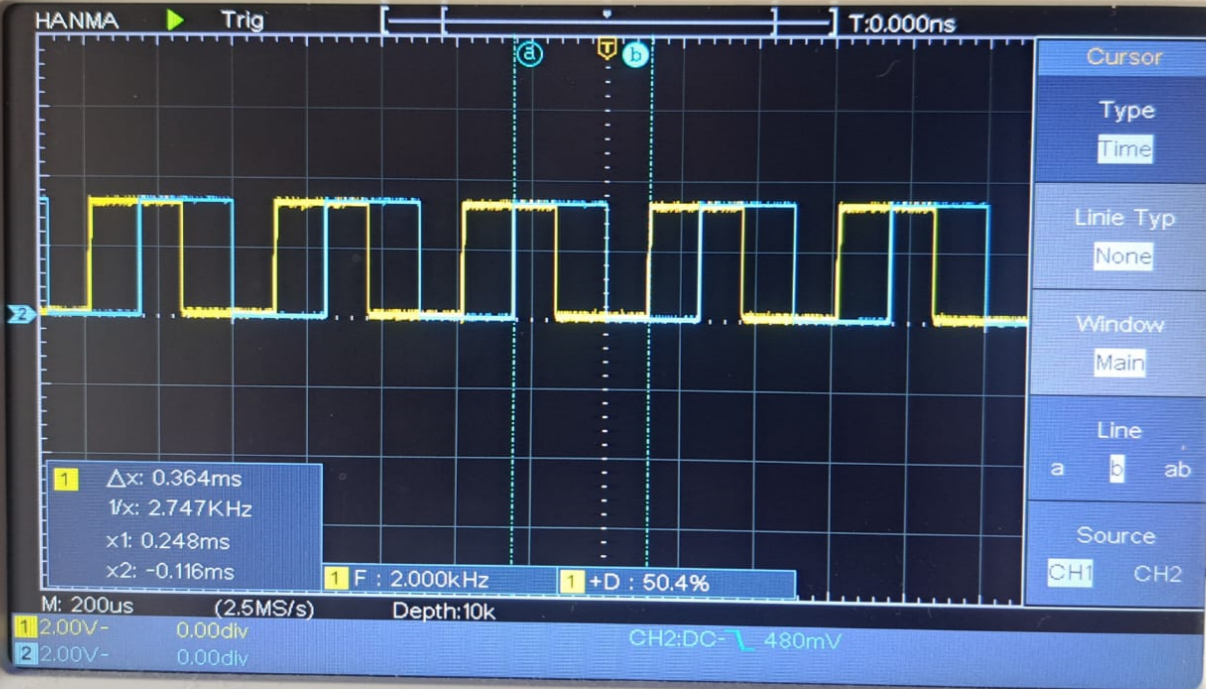
\includegraphics[width=0.5\textwidth]{images/4/4-1/audio-directo.png}
    \caption{Camino de audio sin procesado}
    \label{fig:4-1-dsp-directo}
\end{figure}

Después, probamos por ejemplo a reducir las altas frecuencias y bajar un poco el volumen, obteniendo una salida como la de la \autoref{fig:4-1-dsp-procesado}.

\begin{figure}[h]
    \centering
    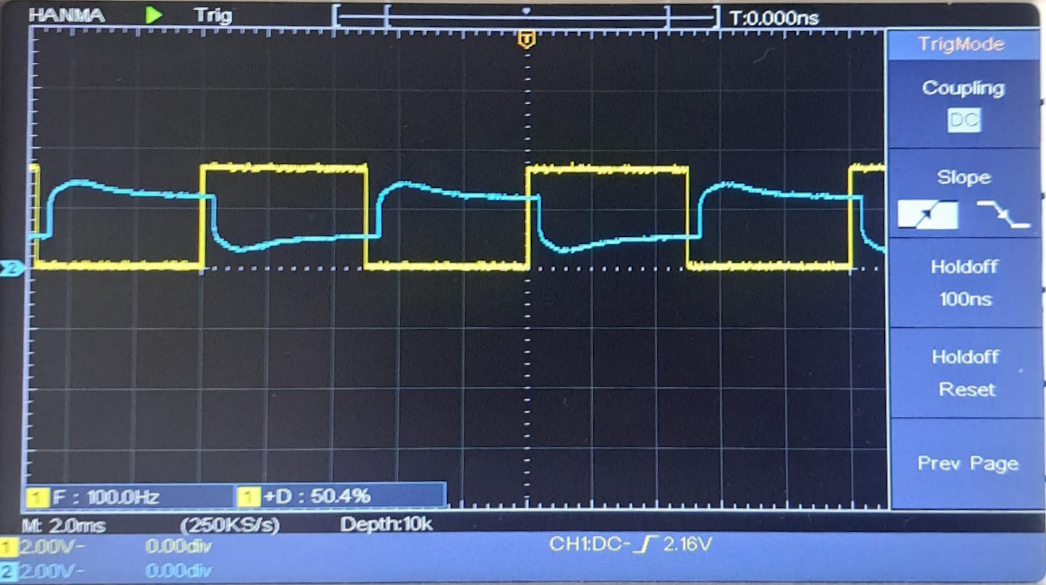
\includegraphics[width=0.5\textwidth]{images/4/4-1/audio-procesado.png}
    \caption{Señal cuadrada procesada digitalmente}
    \label{fig:4-1-dsp-procesado}
\end{figure}
\subsubsection{Test Radio}

El objetivo de esta prueba es la comprobación del correcto funcionamiento del módulo del sintonizador FM. Para navegar entre las direfentes pruebas de este test, se ha utilizador el botón azul (B1) de la propia placa.

Para ello, primero se manda el comando, mediante un \textit{Thread} auxiliar, para encender la radio y se commprueba si se obtiene señal de audio a la salida.

A continuación, se sintoniza una frecuencia concreta y se comprueba, mediante una radio externa, si ambas señales de audio coincide.

Ahora, se realiza un \textit{SeekUp} y se comprueba si la nueva frecuencia sintonizada es mayor a la anterior y si la calidad del audio a aumentado.

De manera análoga, se realiza un \textit{SeekDown} y se comprueba si la frecuencia obtenida es menor a la anterior y también si la calidad de audio aumenta.

A continuación, se intenta sintonizar una frecuencia fuera de rango y se comprueba que solo se obtiene ruido a la salida.

Por último, se manda el comando para apagar la radio y se comprueba que ya no hay señal de auido a la salida.
\subsubsection{Test MP3}

El objetivo de esta prueba es la comprobación del correcto funcionamiento del módulo del reproductor MP3. Para navegar entre las direfentes pruebas de este test, se ha utilizador el botón azul (B1) de la propia placa.

Para ello, primero se inicia la reproducción de una canción concreta y se comprueba si a la salida se escucha esa canción.

Ahora, se manda el comando, mediante un \textit{Thread} auxiliar, el comando que indica la reproducción de la siguiente canción de la lista y se comprueba si se obtiene a la salida.

A continucación, se indica al reproductor que ponga la anteior canción y se comprueba si se escucha dicha canción.

La siguiente comprobación es la puesta en pausa de la canción reproducida, para ella se manda dicho comando y se comprueba que no se obtiene salida.

De forma análoga, se le indica al reproductor que continue con la reproduccón de la canción y se comprueba que se obtiene la canción esperada.

Ahora, se intenta seleccionar una canción que no esté presente en la lista, comprobando que no se obitiene señal a la salida.

Por último, se comprueba el modo \textit{loop}. Para ello se manda el comando indicado y se espera a que termine la canción actual y se comprueba que vuelve a comenzar y, de forma análoga, se indica al reproductor que termine dicho modo y se comprueba, al finalizar la canción actual, que no se obtiene señal a la salida.
\subsubsection{Test RTC}

El objetivo de esta prueba es la comprobación del correcto funcionamiento del módulo RTC.

Concretamente, se prueba si el reloj pasa el tiempo correctamente, si se pasa de minuto y hora adecuadamente y si la fecha se actualiza correctamente.

Implícitamente se comprueba el correcto funcionamiento de la alarma y, además, si la frecuencia a la que se activa es correcta.

También se comprueba si la sincronización con el servidor SNTP es correcta y si la hora actualizada coincide con la fecha y hora actuales.

Por último, se comprueba si los mensajes que envía al programa principal son del tipo correcto y si su contenido es el esperado.
\subsubsection{Test Web}

El objetivo de esta prueba es la comprobación del correcto funcionamiento del módulo del servidor web.

Para ello, se va a dividir este test en dos partes. En la primera, se comprobrá si las peticiones que se generan desde las diferentes páginas web se crean de manera correcta.

Para conseguir esto, se van pulsando sucesivamente todos los botones de todas lás páginas y se comprueba, en el módulo del servidor, si se generan de manera correcta.

También se comprueba si los mensajes que se generan para las diferenctes peticiones creadas son correctos y se envían de forma exitosa al programa principal.

A continuación, se procederá a comprobar si los valores mostrados en las páginas web se actualizan de manera correcta. Para ello, se enviará, desde un \textit{Thread} auxiliar, diferentes modificaciones en los datos mostrado y se comprobrára si se actualizan de manera correcta.

Por último, se comprobará si tanto la hora y la fecha como el consumo se actualizan en tiempo real, implicitamente comprobrando el correcto funcionamiento de las funciones desarrolladas en JavaScript, por lo que se envían durante un cierto periodo de timepo y con una frecuencia de 1Hz, los valores de tiempo, fecha y consumo comprobando que en las diferentes páginas web se muestra de manera correcta.
\subsection{Pruebas hardware}

\subsubsection{Pruebas de la placa de audio}

Para probar la placa de audio, la colocamos sola, alimentándola con una fuente de alimentación de laboratorio, colocando un Jumper entre el terminal de ADC y DAC para no tener en cuenta el procesado digital.

Después, se introduce una señal sinusoidal y se mide la amplitud de salida, calculando la respuesta en frecuencia del circuito. Se recoge una gráfica con la respuesta en frecuencia en decibelios relativos al máximo en la \autoref{fig:4-2-1-respuesta-cascos} (auriculares) y la \autoref{fig:4-2-1-respuesta-altavoces} (altavoces). Cabe destacar que la respuesta dibujada es en decibelios relativos al máximo, por lo que parece que tienen la misma amplitud, pero el altavoz duplica la amplitud de la señal de entrada.

\begin{figure}[h]
    \centering
    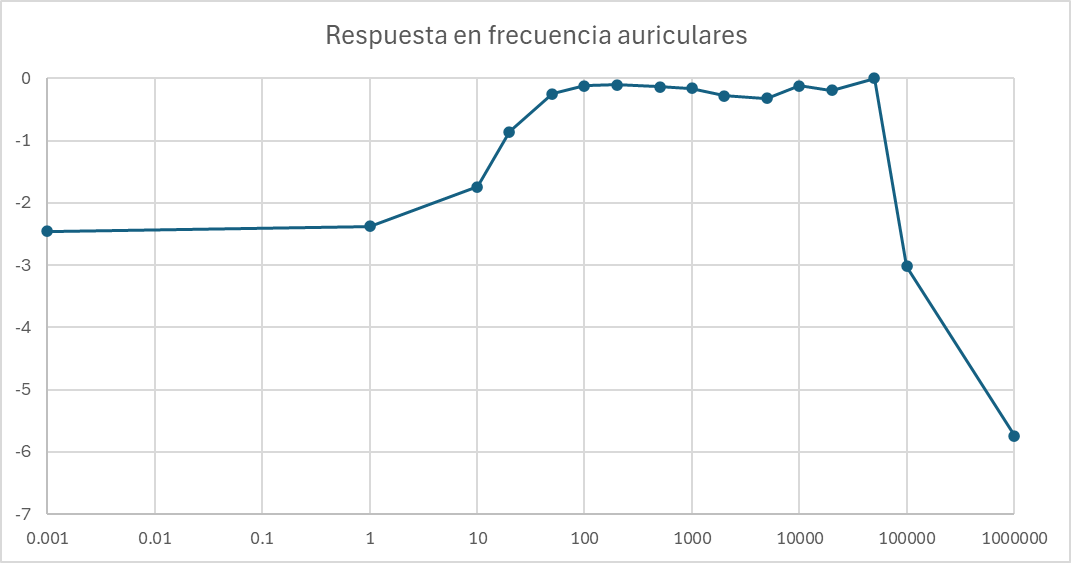
\includegraphics[width=0.5\textwidth]{images/4/4-2/respuesta-auriculares.png}
    \caption{Respuesta del circuito amplificador de auriculares}
    \label{fig:4-2-1-respuesta-cascos}
\end{figure}

\begin{figure}[h]
    \centering
    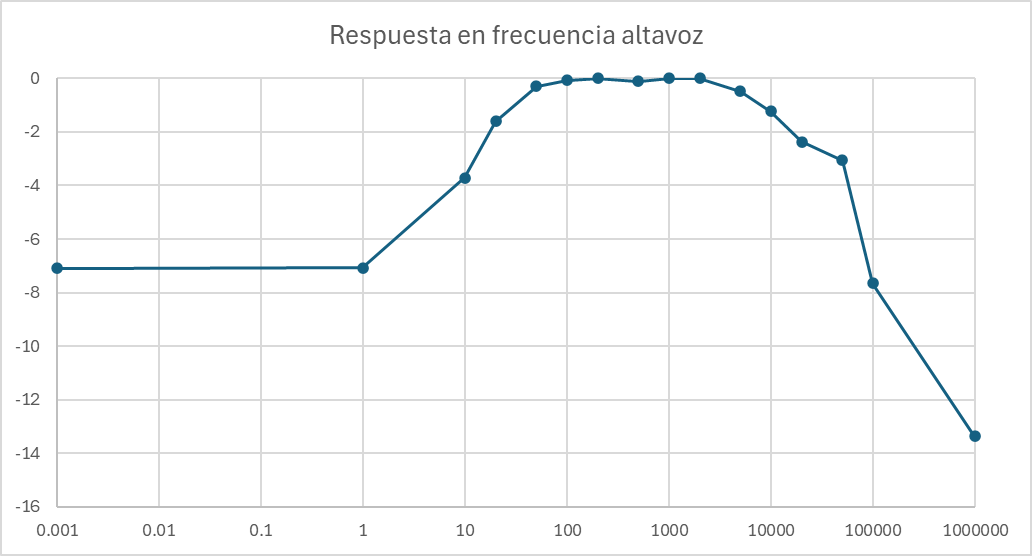
\includegraphics[width=0.5\textwidth]{images/4/4-2/respuesta-altavoces.png}
    \caption{Respuesta del circuito amplificador de altavoces}
    \label{fig:4-2-1-respuesta-altavoces}
\end{figure}

Comprobando el circuito de habilitación, funciona adecuadamente pero a veces se comporta de forma poco consistente al intentar desactivar el circuito cuando está habitado, pero generalmente se comporta correctamente. 

Por otro lado, conectamos distintas cargas y medimos el consumo del circuito, obteniendo los siguientes valores de consumo en función de la impedancia nominal del altavoz. Obtenemos los siguientes valores:
\begin{enumerate}
    \item Auriculates de $~40\ \Omega$: Consumo de $4\ mA$
    \item Altavoz de $8\ \Omega$: Consumo $64\ mA$
    \item Altavoz de $4\ \Omega$: Consumo de $164\ mA$
\end{enumerate}

Además, probando el cambiador de nivel, vemos que consigue una tensión de nivel bajo de $19.78\ mV$ y un $6.99\ V$.

\subsubsection{Pruebas del circuito de alimentación}

Para realizas las pruebas del circuito de alimentación, probamos primero a realizar una descarga y carga de la batería para probar este funcionamiento. Descargamos la batería hasta un valor aproximado de $3.5\ V$ y la volvimos a cargar con nuestro cargador hasta un valor de $4.05\ V$, en el cual la corriente de carga comienza a disminuir y el proceso de carga se ralentiza.

En condiciones normales, la batería carga con una corriente constante de entre $600$ y $700\ mA$, pero disminuye en el tramo final como se comentó en el diseño del circuito. También se ha probado a cargar el circuito a la vez que se carga la batería. Si la fuente tiene suficiente capacidad como para alimentar las dos cosas, hemos comprobado que así lo hace. Hemos probado por ejemplo con una carga de $10\ \Omega$, con lo que el consumo de aproximadamente $
700\ mA$ se suma a la carga obteniendo cerca de $1.5\ A$.

Por otro lado, caracterizamos la regulación de carga para comprobar que nuestro circuito mantuviera la tensión de salida incluso cuando es demandado una gran cantidad de corriente. Se ve que obtenemos un valor de $-39.012 V/A$, o $0.56\%/A$, un buen valor contando con que el consumo aproximado será de medio amperio. Se recoge la gráfica de las medidas en la \autoref{fig:4-2-2-regulacion-carga}.

\begin{figure}[h]
    \centering
    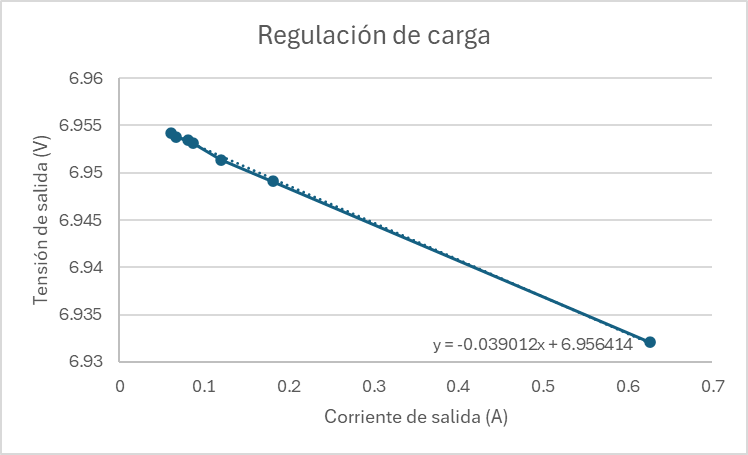
\includegraphics[width=0.5\textwidth]{images/4/4-2/regulacion-carga.png}
    \caption{Regulación de carga del circuito de baterías}
    \label{fig:4-2-2-regulacion-carga}
\end{figure}

Además, comprobamos que los indicadores luminosos funcionan correctamente ya que se enciende el verde cuando se conecta la alimentación y el rojo cuando se está cargando la batería. Al finalizar la carga, se apaga la luz roja y si se enchufa sin estar conectada parpadea el indicador rojo.

Mediante el osciloscopio medimos la tensión de salida del circuito de alimentación, observando que presenta un ruido en muy alta frecuencia, como se puede ver en la \autoref{fig:4-2-2-ruido}. Creemos que este pico de ruido es el culpable de la inestabilidad de los relojes de la placa, pero al colocar condensadores en paralelo no conseguimos reducirlo.

\begin{figure}[h]
    \centering
    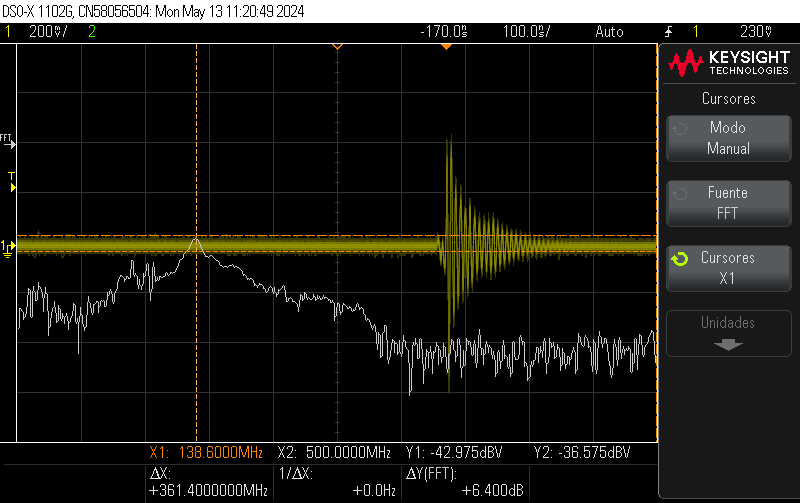
\includegraphics[width=0.5\textwidth]{images/4/4-2/ruido.png}
    \caption{Ruido en la señal de alimentación}
    \label{fig:4-2-2-ruido}
\end{figure}
% \section{Presupuesto}
En la \autoref{tab:presupuesto} se pueden ver los gastos del proyecto.

\begin{table}[H]
    \centering
    \begin{tabular}{lrcr}
    \toprule
    \multicolumn{1}{c}{\textbf{Componente}}  & {\textbf{Precio unitario}}   & {\textbf{Cantidad}} & {\textbf{Precio total}}   \\ \midrule
    \textbf{Batería}                         & {$12.00$ \euro}              & {2}                 & {$24.00$ \euro}           \\ 
    \textbf{CN3768}                          & {$5.89$ \euro}               & {3}                 & {$17.67$ \euro}           \\ 
    \textbf{LDO AMS1117}                     & {$2.05$ \euro}               & {1}                 & {$2.05$ \euro}            \\ 
    \textbf{INA226}                          & {$1.75$ \euro}               & {4}                 & {$7.00$ \euro}            \\ 
    \textbf{PS58F1}                          & {$4.29$ \euro}               & {1}                 & {$4.29$ \euro}            \\ 
    \textbf{LM2596}                          & {$0.61$ \euro}               & {1}                 & {$0.61$ \euro}            \\ 
    \textbf{XL6009}                          & {$0.79$ \euro}               & {1}                 & {$0.79$ \euro}            \\ 
    \textbf{Componentes para el montaje}     & {$20.00$ \euro}              & {N/A}               & {$20.00$ \euro}           \\ 
    \textbf{PCB relé}                        & {$1.00$ \euro}               & {5}                 & {$5.00$ \euro}            \\ 
    \textbf{Componentes relé}                & {$5.00$ \euro}               & {N/A}               & {$5.00$ \euro}            \\ \midrule
    \textbf{Total}                           & { }                          & { }                 & {$86.41$ \euro}           \\ \bottomrule
    \end{tabular}
    \caption{Presupuesto del proyecto}
    \label{tab:presupuesto}
\end{table}
% \section{Equipo de trabajo}

Todos los integrantes hemos colaborado en el diseño de los módulos, pero la responsabilidad principal de cada uno se ha repartido como:

\begin{itemize}
	\item Rubén Agustín Gonzalez: Interfaz de la pantalla de la placa, bajo consumo y uSD.
	\item David Andrino Izquierdo: Esquemático de la alimentación, diseño de las PCBs, módulo de control, protector I2C y procesado digital de señal.
	\item Estela Mora Barba: Esquemático del amplificador de audio, módulo NFC y uSD.
	\item Fernando Sanz Giménez: Módulo RTC, radio, MP3 y web.
\end{itemize}

Las siguientes partes han sido relacionadas de forma conjunta por todos:
\begin{itemize}
	\item Integración del proyecto.
	\item Realización de la memoria.
	\item Powerpoints de las presentaciones.
\end{itemize}

A la hora de colaborar y juntar todas las partes del proyecto, hemos utilizado un repositorio en GitHub \footnote{\url{https://github.com/David-Andrino/ise-rtap}}, con varias ramas creadas para cada miembro. Además, hemos estado trabajando tanto presencial como online, de forma tanto individual como colectiva. Ha habido mucha colaboración entre los miembros del grupo, no solo en lo referente al propio trabajo sino que también de forma emocional. 
% \section{Acrónimos utilizados}

\nocite{*}
%\printbibliography[title={Bibliografía}, heading=bibnumbered]
\todo{Bibliografia}

\begin{appendices}

% Anexo 1. Webench Report
% 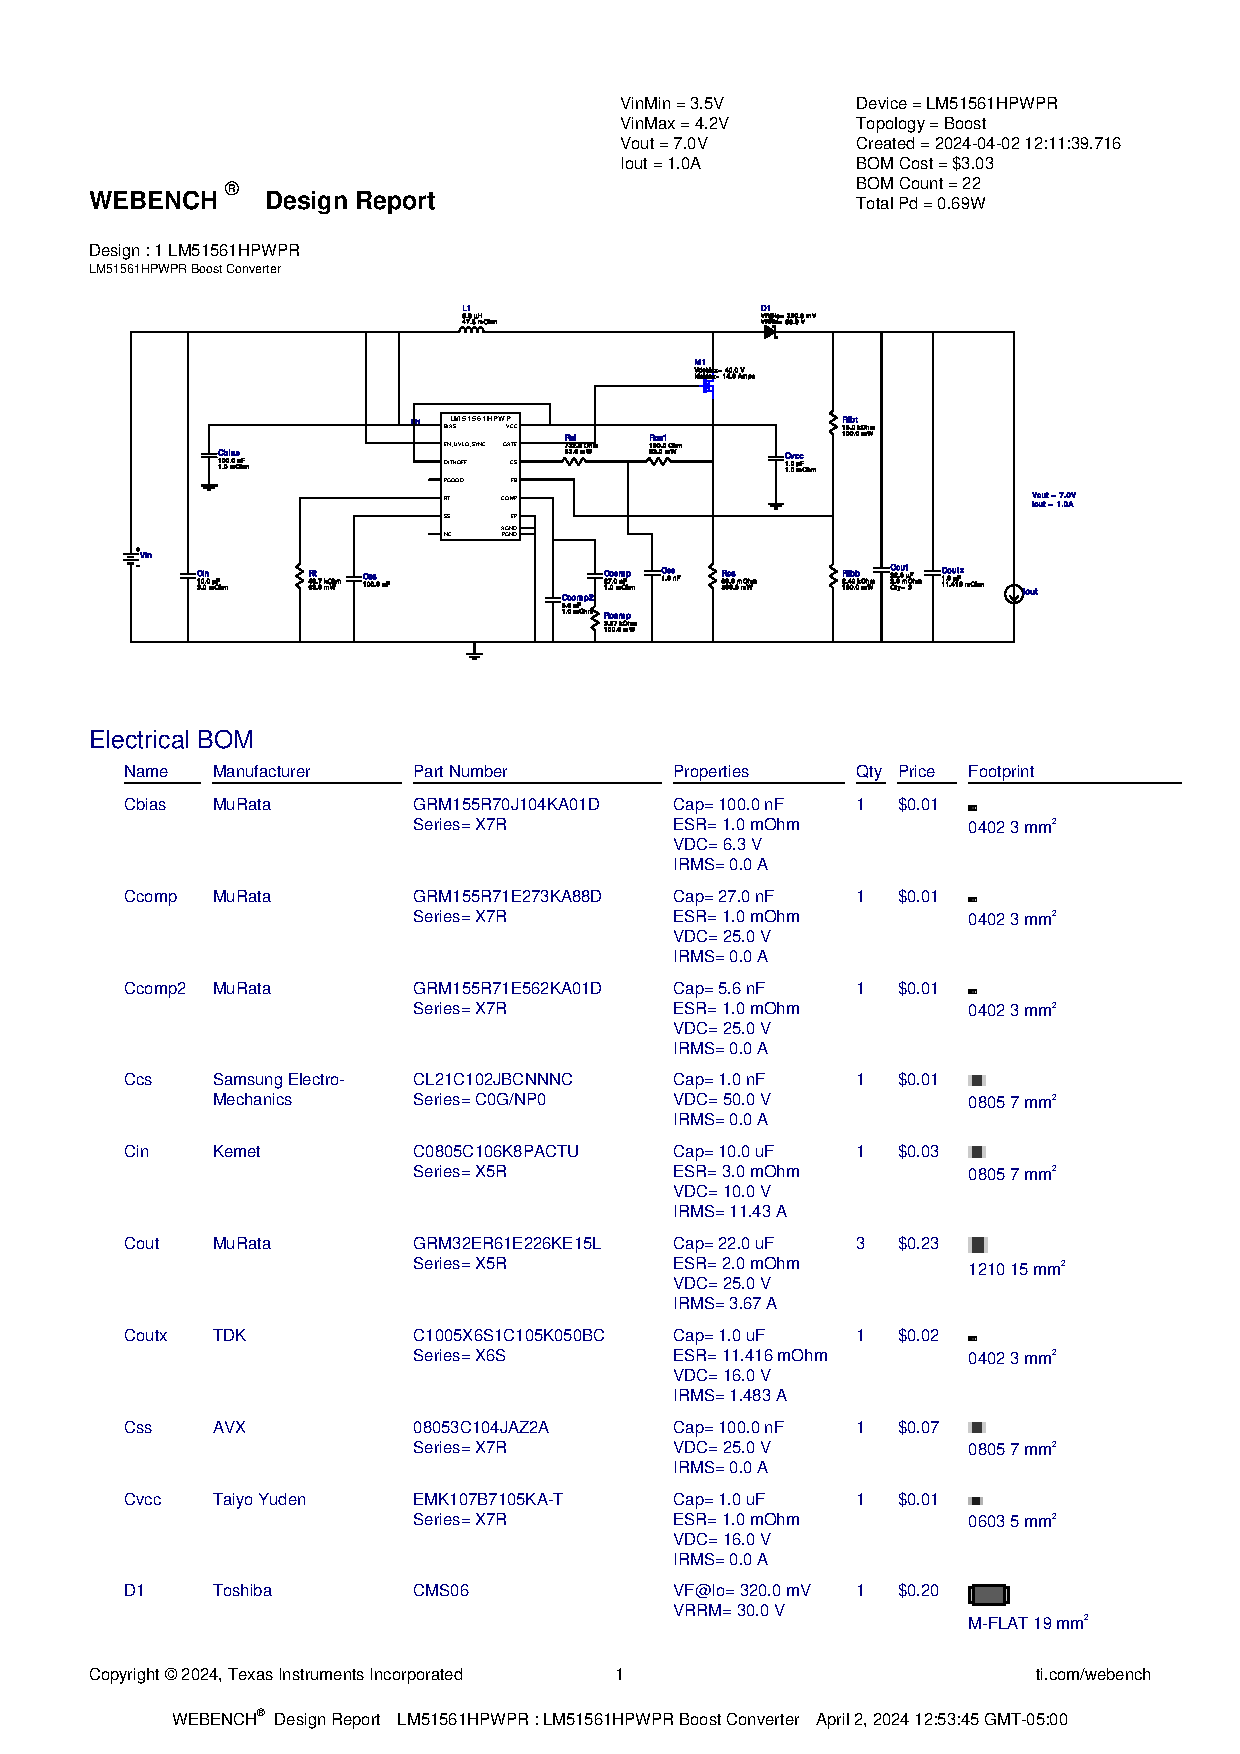
\includepdf[pages=1,offset=0 0,scale=0.8, pagecommand={\section{Webench Design Report}\label{anexo:webench-report}}]{./files/8-Anexos/WebenchDesignReport.pdf}
% \includepdf[pages=2-7,offset=0 0,scale=0.8, pagecommand={}]{./files/8-Anexos/WebenchDesignReport.pdf}

\end{appendices}



\end{document}
